%  $Id::                                                                $

\documentclass[11pt,a4paper]{report}
\usepackage{epsfig,colordvi,latexsym}
\pretolerance=10000
\topmargin=0mm
\headheight=0mm
\headsep=8mm
\textwidth=170mm
\textheight=240mm
\footskip=15mm
\oddsidemargin=0mm
\evensidemargin=-12mm
\parskip=3mm
\parindent=0mm

\setcounter{secnumdepth}{3}
\newcommand{\PS}{\mbox{\it PROCESS\/ }}
\newcommand{\PSD}{\mbox{\it PROCESS}\@.\/ }
\newcommand{\PSC}{\mbox{\it PROCESS},\/ }
\newcommand{\INCLUDE}{\mbox{\tt INCLUDE }}
\newcommand{\COMMON}{\mbox{\tt COMMON }}

\newcommand{\setheader}[1]
 {\markright{\rlap{\lower0.8ex\hbox to\textwidth{\hrulefill}}{\bf#1}}}
\newcommand{\mychapter}[1]{\small\normalsize
 \setcounter{footnote}{0}
 \chapter{#1}
 \pagestyle{myheadings}
 \setheader{Chapter \thechapter\hspace{0.8em}#1}}
\newcommand{\myappendix}[1]{\small\normalsize
 \setcounter{footnote}{0}
 \chapter{#1}
 \pagestyle{myheadings}
 \setheader{Appendix \thechapter\hspace{0.8em}#1}}

\begin{document}

\footnotesize
\hfill T\&M/PKNIGHT/PROCESS/MANUAL

\vspace*{4cm}
\begin{center}
\Huge A User's Guide\\ to the \\ PROCESS Systems Code\\
~\\ \LARGE P.\ J.\ Knight\\
~\\ \Large EURATOM/CCFE Fusion Association\\
Culham Science Centre, Abingdon, Oxon, OX14 3DB, UK
\end{center}

\vfill
\footnotesize
\verb?$Date::                                              $?
\hfill
\verb?$Revision::     $?

\normalsize
\tableofcontents

\mychapter{Introduction}
\label{chap:intro}

\section{Rationale}

The \PS systems code is being developed to provide an integrated and
self-consistent treatment of the physics, engineering, economic, safety and
environmental characteristics of fusion power plants. This will enable issues
of the feasibility and safety advantages of different power plant designs to
be systematically explored.

During the course of studies of a proposed fusion power plant, there may be
times when questions of the following type arise:
\begin{quote}
Are the machine's physics and engineering parameters consistent with one
another?

Which machine of a given size and shape produces the cheapest electricity?

What is the effect of a more optimistic limit on the plasma beta on the amount
of auxiliary power required?
\end{quote}

Questions such as these are extremely difficult to answer, since the large
number of parameters involved are highly dependent on one another.
Fortunately, computer programs have been written to address these issues, and
\PS is one of them.

Suppose that an outline power plant design calls for a machine with a given
size and shape, which will produce a certain net electric power.  There may be
a vast number of different conceptual machines that satisfy the problem as
stated so far, and \PS can be used in non-optimisation mode to find one of
these whose physics and engineering parameters are self-consistent. However,
the machine found by \PS in this manner may not be possible to build in
practice --- the coils may be overstressed, for instance, or the plasma
pressure may exceed the maximum possible value. \PS contains a large number of
constraints to prevent the code from finding a machine with such problems, and
running the code in optimisation mode forces these constraints to be met. The
number of possible conceptual machines is thus considerably reduced, and
optimisation of the parameters with respect to (say) the cost of electricity
will reduce this number to a minimum (possibly one).

Formally then, \PS is a systems code that calculates in a self-consistent
manner the parameters of a fusion power plant with a specified performance,
ensuring that its operating limits are not violated, and with the option to
optimise a given function of these parameters.

It would not be fair to call \PS a fusion power plant design code, as this
implies that a great deal of complexity would need to be present in each and
every model describing one of the component systems. Such complexity is,
however, incompatible with the code's iterative approach to solving the
optimisation problem, since this requires repeated evaluation of the same
(large number of) expressions. This is not to say that the models employed by
the code are oversimplified --- in general they represent good numerical
estimates of present theoretical understanding, or are fits to experimental
data. \PS provides a useful overall description of how a conceptual and
feasible power plant may look.

\section{History}

\PS is derived from several earlier systems codes, but is largely based on the
TETRA (Tokamak Engineering Test Reactor Analysis) code~\cite{tetra} and its
descendant STORAC (Spherical TOrus Reactor Analysis Code)~\cite{storac}, which
includes routines relevant to the tight aspect ratio class of tokamaks. These
codes, and much of the original version of \PS itself, were written by
personnel at Oak Ridge National Laboratory in Tennessee, USA, with
contributions from a number of other laboratories in the USA\@. In addition,
many of the mathematical routines have been taken from a number of different
well-established source libraries.

Since the code is descended from such a wide range of sources, its structure
was initially not ideal from the programmer's viewpoint.  Non-standard
practices and inconsistent layout within the code could have led to
difficulties in modifying, interpreting and indeed running the code. A great
deal of effort has therefore been expended at Culham since the code's arrival
from ORNL to improve this situation, with the code being given a complete but
careful upgrade, routine by routine. A {\em single}\/ master copy of \PS now
exists, the details of which are described here. The culmination of the work
to improve the usability of the code is this User Guide, which hopefully will
be of assistance to all users of \PSC whether they are planning to modify or
run the code, or are simply trying to understand what the code aims to
achieve.

As with all active research codes, \PS will continue to be developed for some
time. As explained earlier in this introduction, the code will be used as the
basis of power plant environmental and safety studies by the inclusion of
further models and constraints. This User Guide is updated regularly to ensure
that the documentation is consistent with the latest version of the code.

\section{Layout of the User Guide}

The User Guide is divided into a small number of logically separate units,
each one of which provides specific information on a given topic. It depends
on the user's motive for referring to the manual as to which chapter will be
the most useful, although hopefully the style and structure adopted will allow
one to browse through without difficulty.

Chapter~\ref{chap:overview} provides an overview of the program and the
machine that is modelled by it. Chapter~\ref{chap:models} goes into slightly
more detail, and discusses the various physics and engineering models that are
used within the code to describe the power plant systems.
Chapter~\ref{chap:run} describes how to run the program from scratch, and
provides a number of hints and suggestions to bear in mind when the code does
not find a feasible machine. Chapter~\ref{chap:modify} shows how to modify the
code in specific ways, for example how extra constraints and variables should
be added to the code. Appendices~\ref{app:infile1} and~\ref{app:infile2}
contain example input files for \PS in non-optimisation and optimisation
modes, respectively. Finally, Appendix~\ref{app:doc} contains references for
useful Work File Notes~\cite{PWF} that provide information about the code
status, its location, and other details relating to the implementation of \PS
to date.

This manual has been written in such a way as to (a) lead a new user of \PS
into a clear understanding of the code's concepts, structure and models, and
(b) help a more experienced user to set up and run the code efficiently and
quickly. Potential users of \PS need only a basic knowledge of potential
fusion power plants, and access to the code itself. No specialised knowledge
in computers or computing is required.

\mychapter{Program Overview --- The Fundamentals}
\label{chap:overview}

This chapter presents the reader with a first glimpse into the world of \PSD
It is clearly important when one is trying to get to grips with a code of the
proportions of \PS to be able to visualise the main aspects of the device
being simulated at an early stage, without too much detail obscuring the
overall picture. Similarly it is important to provide the potential users with
an overview of the code structure and its operation before they embark on a
closer study. The aim of this chapter is to aid this visualisation by
presenting a brief description of the machine, its subsystems and the code
layout in simple, general terms. Chapter~\ref{chap:models} will provide users
with more detail about how to customise the models and parameters mentioned
here.

\section{The Machine}

A natural starting point for a systems code manual is the description of the
system itself. In this case, the (default) system is a tokamak fusion power
plant, modelled using a large number of equations based on knowledge of the
underlying physics and engineering models of each subsystem of the machine. As
will be emphasised later the bulk of the program is ordered into modules
roughly corresponding to each of the subsystems, so an early attempt at
familiarising the reader with them will hopefully be of some benefit.

\subsection{Radial and Vertical Build}
Figure~\ref{fig:build1} shows schematically the layout of a typical tokamak as
modelled by \PSD This is the so-called `build' of the machine --- the relative
locations of the major components. Their positions are referenced to the
$(R,Z)$ coordinate system, where $R$ is the radial distance from the vertical
centreline (axis) of the torus, and $Z$ is the vertical distance from the
equatorial midplane, about which the machine is assumed to be up-down
symmetrical. Components are often referred to as being `inboard' or
`outboard', which simply means that they lie at a radius $R$ less than or
greater than $R_0$, respectively, where $R_0$ is the plasma major radius ({\tt
rmajor}).

\begin{figure}
\centerline{\epsfig{file=BUILD1.ps,width=160mm,height=160mm,
bbllx=0mm,bburx=200mm,bblly=0mm,bbury=200mm,clip=}}
\vspace{-12mm}
\caption[build1] {\it Schematic diagram of the fusion power core of a typical
tokamak power plant modelled by \PSC showing the relative positions of the
components. The numbers shown in the PF coil blocks are the values of the {\tt
ipfloc} switch for that block.}
\label{fig:build1}
\end{figure}

Figure~\ref{fig:build2} shows the \texttt{Fortran} variables that describe the
thicknesses and positions involved. It must be emphasised that these two
figures are very much schematic, otherwise they could become slightly
misleading. For the sake of clarity the thicknesses are not drawn to scale,
and the space labelled as the divertor does not indicate in any way the actual
shape of that component. The cryostat acts as a dewar or vacuum vessel, and is
therefore continuous in reality, enclosing all of the components within
it. Only in the code's build calculation is there an apparent gap in the
cryostat beneath the top of the TF coil.

\begin{figure}
\centerline{\epsfig{file=BUILD2.ps,width=160mm,height=160mm,
bbllx=0mm,bburx=200mm,bblly=0mm,bbury=200mm,clip=}}
\vspace{-12mm}
\caption[build2] {\it Schematic diagram of the fusion power core of a typical
tokamak power plant modelled by \PSC showing the variables used to define the
thicknesses of the components. The arrowed labels adjacent to the axes are the
total `builds' to that point. The precise locations and sizes of the PF coils
are calculated within the code.}
\label{fig:build2}
\end{figure}

Most of the thicknesses shown in Figure~\ref{fig:build2} are input parameters,
so are not changed during the course of the simulation.  The rest are
calculated by the code during execution. In addition, some of the component
sizes can be used as {\it iteration variables}\/ (see
Section~\ref{sec:itvars}) to help in the optimisation process.

\subsection{Principal Components}

\subsubsection{Plasma}
Arguably, the most important component of the machine is the plasma
itself. This is assumed to have an up-down symmetric, double null
configuration, with elongation and triangularity specified by the user. A
great number of physics models are coded within \PS describing the behaviour
of the plasma parameters such as its current, temperature, density, pressure,
confinement etc., and also the various limits that define the stable operating
domain.

\subsubsection{Scrape-off Layer}
The region directly outside the last closed flux surface of the plasma is
known as the scrape-off layer, and contains no structural material.  Plasma
entering this region is not confined and is removed by the divertor. \PS
treats the scrape-off layer merely as a gap.

\subsubsection{First Wall}
The first wall acts as a physical barrier protecting the rest of the machine
from the hot plasma. Due to its hostile environment the first wall has only a
short lifetime and therefore needs to be replaced regularly. Its stainless
steel structure is cooled either by gaseous helium or by pressurised water.

\subsubsection{Divertor}
The divertor provides a means of removing plasma reaching the scrape-off layer
and heavy ions that are ejected from the first wall.  Two divertors are
assumed in the \PS tokamak, placed symmetrically above and below the plasma
(N.B.\ see Section~\ref{sec:divmod}). The principal outputs from the code
are the divertor heat load, used to determine its lifetime, and its peak
temperature. The divertor is cooled either by gaseous helium or by pressurised
water.

\subsubsection{Blanket}
The blanket performs a number of tasks. An incoming neutron from a
deuterium-tritium (D-T) fusion reaction in the plasma loses energy in the
blanket. This energy is removed by the blanket coolant and used to produce
electricity. The neutron may also react with a lithium nucleus present in the
blanket to produce a tritium nucleus which can be re-used as fuel. The
competing requirements of heating and tritium synthesis mean that a neutron
multiplier must be present, to ensure balance between tritium destruction and
creation. The blanket therefore contains beryllium to fulfil this
purpose. Again, the blanket has a relatively short lifetime because of the
high neutron fluence. Steel and vanadium may be used as structural materials
within the blanket, which is cooled either by gaseous helium or by pressurised
water.

\subsubsection{Shield}
The stainless steel shield reduces the neutron flux reaching the TF coils and
beyond. This minimises the radiological impact of the neutrons, and their
heating of the TF coils which, if superconducting, need to remain at liquid
helium temperatures. The shield is cooled either by gaseous helium or by
pressurised water, and as with the blanket the energy deposited in the coolant
is used to produce electricity.

\subsubsection{TF Coils}
The toroidal field (TF) coils can be either resistive or superconducting. In
the superconductor model, the CICC (Conductor In Cable Conduit) structure
shown in Figure~\ref{fig:CICC} is used, and the coils are cooled using a
liquid helium cryogenic system. Among the TF coil parameters calculated by the
code are the maximum allowable current density, the stresses on the structure,
the energy stored and the magnetic field produced by the coils.

The current in the TF coils must be sufficient to produce the right toroidal
field at the centre of the plasma. The field falls off at a rate $1/R$, with
the peak value occurring at the outer edge of the inboard portion of the TF
coil ($R_{\mbox{\scriptsize max TF}} = \mbox{\tt rbmax}$). The maximum TF coil
current depends on the field it produces and the allowable current density.

Each TF coil is defined in the $(R,Z)$ plane by four circular arcs of
different radius, which create a D-shaped profile. Because of the finite
number of TF coils used in a tokamak (typically around 20), the toroidal field
has a ripple introduced into it, the amplitude of which can be limited to a
few per cent by the code by adjusting the outboard gap thickness (labelled
{\tt gapsto} in Figure~\ref{fig:build2}).  Ports are often necessary for
auxiliary power systems etc., and the gaps between adjacent TF coils can be
made large enough to accommodate such equipment.

\begin{figure}
\centerline{\epsfig{file=CICC.ps,width=160mm,height=160mm,
bbllx=0mm,bburx=210mm,bblly=0mm,bbury=210mm,clip=}}
\vspace{-12mm}
\caption[CICC]
{\it Schematic diagram of the cross-section of a superconducting TF coil,
showing the CICC (Conductor In Cable Conduit) construction. The cable space
contains superconducting filaments and circulating liquid helium coolant.}
\label{fig:CICC}
\end{figure}

\subsubsection{Bucking Cylinder}
The bucking cylinder provides some strength to the inboard TF coil
structure. If the TF coils are superconducting, the bucking cylinder is cooled
by the cryogenic system.

\subsubsection{Cryostat}
The cryostat acts as a dewar and vacuum vessel, and is used to cool those
components that need to operate at liquid helium temperatures. These include
any superconducting (TF or PF) coils, the inter-coil structure and the bucking
cylinder. \PS calculates the cryogenic power load and the resulting heat
exchanger requirements. As stated earlier, the build picture in
Figure~\ref{fig:build1} is slightly misleading in that the cryostat completely
encloses the components within it --- there is no large gap beneath the TF
coil as is the case in Figure~\ref{fig:build1}.

In addition to this (inner) cryostat, an external cylindrical dewar encloses
the whole of the tokamak.

\subsubsection{PF Coils}
The poloidal field (PF) coils can be either resistive or superconducting, and
are used initially to cancel the vertical field produced at the centre of the
plasma by the OH coil during start-up, and then to maintain the plasma
position and shape during the flat-top period. The positions and sizes of the
PF coils are partly input, and partly calculated after consideration of the
required currents and allowable current density. The PF coils are generally
grouped into up-down symmetric pairs, and each group can be placed in one of
three regions, either vertically above (and below) the OH coil ({\tt
ipfloc(i)=1}), vertically above (and below) the TF coil ({\tt ipfloc(i)=2}),
or radially outside the TF coil ({\tt ipfloc(i)=3}).

The PF coil currents vary as a function of time during the tokamak operation
as indicated in Figure~\ref{fig:current_vs_time}.

\begin{figure}
\centerline{\epsfig{file=IVST.ps,width=160mm,height=160mm,
bbllx=0mm,bburx=200mm,bblly=0mm,bbury=200mm,clip=}}
\vspace{-12mm}
\caption[IvsT]
{\it Plot showing schematically the current waveforms for the plasma, a
typical PF coil, and the OH coil.}
\label{fig:current_vs_time}
\end{figure}

\subsubsection{OH Coil}
The ohmic heating (OH) coil is a PF coil used primarily during start-up (but
also during the burn phase) to create and maintain the plasma current by
inductive means. Swinging (changing) the current through the OH coil causes a
change in the flux linked to the plasma region, inducing a current in it. \PS
calculates the amount of flux required to produce the plasma current, and also
the amount actually available. The code measures the magnetic flux in units of
Volt-seconds ($=$ Webers). The OH coil is sometimes referred to as the central
solenoid, and can be either resistive or superconducting.

\subsubsection{Auxiliary Power Systems}
The use of purely inductive current drive leads to pulsed plant operation
because of the limited flux swing that can be achieved using the OH coil. This
poses problems due to the fact that fatigue failures may result, and there
would also be a need for thermal storage to maintain a level supply between
pulses. However, the plasma current can also be produced and maintained
(partially or wholly) using non-inductive means which, in principle, removes
this restriction. \PS contains a number of auxiliary current drive schemes,
including various RF methods (Lower Hybrid, Electron Cyclotron, and Ion
Cyclotron (Fast Wave) current drives) and also Neutral Beam current drive
systems. The code calculates the efficiency and the resulting power
requirements of the chosen system.

\subsubsection{Structural Components}
Structural components are required to provide support for the fusion power
core systems against gravity and the magnetic forces that will be encountered
during operation. The required structural masses and their costs are
calculated.

\subsubsection{Power Conversion and Heat Dissipation Systems}
The \PS power plant takes into account all the systems required to perform the
necessary conversion of fusion power to electricity, from the coolant systems
in the plant components to the heat exchangers and turbines.
Figure~\ref{fig:pwrconv} shows schematically the overall power transfer
mechanisms used by the code.

\begin{figure}
\centerline{\epsfig{file=PWR.ps,width=160mm,height=160mm,
bbllx=0mm,bburx=200mm,bblly=0mm,bbury=200mm,clip=}}
\vspace{-12mm}
\caption[PWRCONV]
{\it Schematic diagram showing the power conversion mechanisms used in \PS
\cite[Note 0166]{PWF}.}
\label{fig:pwrconv}
\end{figure}

\subsubsection{Vacuum Systems}
The vacuum system is used for four different processes. Firstly, before plasma
operations the chamber must be evacuated to remove outgassed impurities from
the structure. Secondly, the chamber must be re-evacuated between burn
operations. Thirdly, helium ash must be removed to prevent it from diluting
the fuel. Finally, deuterium and tritium is removed on a steady state
basis. \PS calculates the parameters of a vacuum system that satisfy all four
requirements, with the option of either turbo pumps or cryo pumps being used.

\subsubsection{Buildings}
The volume and ground area of all the various buildings on a power plant site
are included in the \PS calculations for the benefit of the costing
algorithms.

\subsection{Tight Aspect Ratio Tokamaks}

\PS has the ability to perform studies on tokamaks in the low aspect ratio
regime (major radius $\leq 2 \times$ minor radius). The physics and
engineering issues~\cite{tart} associated with these machines are somewhat
different from those of conventional aspect ratio, and this is reflected by
the following special models~\cite{storac} in \PSD
\begin{enumerate}
\item The inboard build of a TART is very different from that in a
conventional tokamak. There is no inboard blanket (and possibly no inboard
shield), and the inboard TF coil legs are replaced by a single centrepost.
\item The centrepost is constructed from copper (as are the outboard TF coil
sections), and is tapered so that it is narrowest at the midplane of the
device. The parameters of the centrepost coolant system are calculated by \PSC
including the pump pressure, maximum temperature and pipe radius.
\item A gaseous divertor model is used, and a simple divertor heat load
calculation is employed.
\item A simple PF coil current scaling algorithm is available for use with the
TART option.
\item The plasma shaping terms (elongation and triangularity) can be
calculated directly given the aspect ratio.
\item Among the physics models that differ from those relevant to conventional
aspect ratio machines are (i) the bootstrap current fraction, (ii) the Troyon
beta limit, and (iii) the neutron heating of the centrepost.
\end{enumerate}
Since \PS is set up by default to deal with conventional aspect ratio
machines, TART power plants will only be referred to briefly in the rest of
this manual.

\subsection{D-$^3$He Tokamaks}

In addition to the standard deuterium-tritium fusion reaction
(Equation~\ref{eq:d-t}), \PS can also investigate power plants that utilise
the deuterium-$^3$helium reaction (Equation~\ref{eq:dhe3}). The fusion
reaction rate is significantly different from that for D-T fusion, and the
power flow from the plasma is modified since charged particles are produced
rather than neutrons.

D-$^3$He tokamak power plants do not include blankets, because of the near
absence of neutrons leaving the plasma, and the fact that no tritium needs to
be produced for fuel.

\subsection{Pulsed Plant Scenario}

If the plasma current is not to be driven by purely non-inductive means, it is
necessary to operate the plant in a pulsed manner as the current swing in the
OH/PF coils cannot be continued indefinitely. \PS can perform a number of
calculations relevant to a pulsed power plant, as summarised below.

\subsubsection{Thermal Cycling Package}
This performs calculations on the first wall of the machine. Evaluation of the
mechanical and thermal stresses on this component lead to a measure of the
maximum number of cycles to which the first wall can be subjected, and hence
to the minimum allowable length of each reactor cycle for a specified first
wall lifetime. The thickness of the first wall is constrained to lie within
lower and upper bounds, which ensures that it can withstand the internal
coolant pressure and the peak temperature and neutron fluence.

\subsubsection{OH Coil Swing Time}
This calculation ensures that the plasma current ramp rate during start-up is
prevented from being too high, as governed by the requirement to maintain
plasma stability in $l_i$ - $q_\psi$ space.

\subsubsection{Burn Time}
The length of the burn time is calculated from the surplus volt-seconds
available from the OH/PF coil system during the plasma burn phase, after the
flux required during the plasma start-up is taken into account.

\subsubsection{Start-up Power Requirements}
The minimum auxiliary power required during the start-up (ignition) phase is
calculated on the basis of a POPCON analysis. Ignition is accessed via the
so-called Cordey Pass (the path in plasma density--temperature space which
minimises the power requirement) and the code ensures that there is sufficient
auxiliary power to accommodate this. In fact, this calculation is very
CPU-intensive, so the relevant routine is not called at present. In practice,
the auxiliary power tends to exceed the minimum allowable value anyway,
without any need to constrain it to do so.

\subsubsection{Thermal storage}
Three options for providing the thermal storage required to maintain the
machine's output during the off-periods are available. The first relies on the
thermal storage inherent in the machine's steam cycle, the second incorporates
an extra boiler to boost the thermal storage, and the third relies on a large
stainless steel block acting as the thermal storage medium. The costs of these
three options are added to the relevant cost accounts.

\subsection{Safety and Environment Models}
At present, the neutronics, activation and inventory calculations comprise the
safety and environment models in the code. These will be extended as a result
of forthcoming work.

\subsubsection{Neutronics}
The neutronics module predicts the neutron flux spectra in the inboard and
outboard first wall and blanket components. The spectra are based on a
simplified tokamak device that has a fixed ratio ($=1.5825$) between the
outboard blanket thickness and the inboard blanket thickness, and are scaled
according to the actual thickness of the outboard blanket. This relatively
limited, single-parameter approach is expected to be replaced by a more
general method, which should allow a more accurate portrayal of the device
being modelled by \PSD

\subsubsection{Activation and Inventory Information}
The code evaluates the consequences of exposing the power plant's materials to
the calculated neutron fluxes, subject to the limitations imposed by the
neutronics module. A library of neutron cross-sections and decay data is used
to calculate the total activity, gamma-ray dose rate and decay heat output due
to the materials' exposure to neutrons, both at the end of the plant's life
and at a time 100 years later. These values are relevant to decommissioning
and disposal studies, and additional parameters that can be obtained from the
nuclide inventory will also be included as the need arises.

\subsection{Stellarator Model}
The code has the ability to perform calculations based on the physics and
engineering of a stellarator, which, although being a toroidal device, is
radically different in a number of ways from a tokamak.

The model is derived from two main sources; the physics is based on that
assumed by the U.S.\ stellarator reactor study group~\cite{USSRSG}, and the
coil set is scaled from the proposed Wendelstein VII-X design, a modular
advanced stellarator with a 5-period Helias configuration~\cite{W7X}.

\subsubsection{Physics Models}
Much of the physics is identical to that for tokamaks, including the plasma
composition, fusion power considerations and energy conversion and transport
within the plasma. However, some physics topics do differ between stellarators
and tokamaks:
\begin{enumerate}
\item Plasma current scaling: Stellarators have zero plasma current, so no
current scalings are required.
\item Heating/current drive: Stellarators require no current drive, although
provision for auxiliary heating does need to be present.
\item Density and beta limits: Stellarator-relevant plasma limits are
available within the code.
\item $\tau_E$ scaling laws: Three confinement time scaling laws
relevant to stellarators are present, in addition to those that apply to
tokamaks.
\end{enumerate}

\subsubsection{Machine Configuration}
There are a large number of possible stellarator configurations. The one
chosen for the \PS model is based on the {\bf HELI}cal {\bf A}dvanced {\bf
S}tellarator (Helias) concept, in which all the coils resemble distorted,
non-planar TF coils --- no helical coils or tokamak-like PF coils are present.
This approach was chosen because the Helias is the most promising stellarator
concept for a power plant, with a modular engineering design and optimised
plasma, MHD and magnetic field properties~\cite{HSR}. Furthermore, this choice
also enabled the coil engineering issues to be coded easily by simply
modifying the existing \PS superconducting TF coil model. The coil geometry is
scaled from the proposed Wendelstein VII-X device, which is based on a five
field-period Helias configuration.

Since a stellarator is inherently non-axisymmetric, the build of the \PS
stellarator is defined in terms of the mean thicknesses of components. This
allows the code to use the existing algorithms for the surface areas, volumes
and masses of the plasma and the machine's structural materials, without
introducing unacceptably large errors in the calculated values.

All items external to the fusion power core (buildings, turbines, power
conversion systems, etc.) remain unchanged.

\subsubsection{Modelling of Stellarator Coils}
The stellarator coils are assumed to be superconducting --- no resistive coil
calculations are performed.  The overall calculations on the coils are largely
unchanged, as the present superconducting routines still apply. However, the
geometry of the coils is different from that for tokamak TF coils, so some
modification has been necessary.

Firstly, the inboard legs do not form a continuous ring of material on the
midplane --- adjacent coil cases do not touch. This causes the calculation of
the inboard coil conductor area to change, and also the shape of the winding
pack cross-section. This is assumed to be rectangular for the stellarator
coils, rather than the complicated two-step cross-section assumed for tokamaks
(see Figure~\ref{fig:stell1}).

\begin{figure}
\vspace*{180mm}
\caption[tosh]{\it TF coil inboard leg cross-sections for tokamak and
stellarator devices (Fig.~1, Work File Note~F/RS/CIRE5523/PWF/0248).}
\label{fig:stell1}
\end{figure}

Secondly, the shape of the coils in the poloidal plane is not D-shaped, and
varies from coil to coil. This has a number of implications, not least on the
length (and hence total mass and cost) of the coil set. In order to model a
set of realistically-shaped stellarator coils, geometry $(\theta,\phi)$ data
were taken from the Wendelstein VII-X coil set design~\cite{W7X} and these are
fitted onto the surface of a helically-modulated torus whose radii scale with
the machine's desired radial build. The total length of the coils is then
calculated. For simplicity, the poloidal cross-section of the torus onto which
the coils are mapped is assumed to be elliptical, with the major axis of the
ellipse rotating with toroidal angle. This is only a rough estimate of the
true cross-sectional shape; however the resulting coil set is a fair
approximation to the true case (see Figure~\ref{fig:stell2}).

\begin{figure}
\vspace*{180mm}
\caption[tosh]{\it Comparison between (a) the Wendelstein VII-X coil set and
(b) the PROCESS stellarator coil set. The inboard sections of the PROCESS
coils are plotted with circular symbols for clarity (Fig.~2, Work File
Note~F/RS/CIRE5523/PWF/0248).}
\label{fig:stell2}
\end{figure}

In order to use the existing routines for calculating the stresses in the
coils, it is necessary to describe the poloidal variation of the coil shape
using four circular arcs. For the purpose of these calculations the coil shape
is assumed to be elliptical.

\subsubsection{Other Systems}
Many of the fusion power core systems are assumed to have the same
characteristics as for a tokamak device, including the blanket, divertor,
cryogenic and vacuum systems. Of these, only the calculations for the divertor
are likely to be inaccurate, as in a large stellarator device the divertor is
expected to be helical rather than axisymmetric as is the case in tokamaks.

\subsubsection{Code Modifications}
The stellarator model impacts the rest of the code in such a way as to
minimise the effort that would be required in the future to modify or remove
the stellarator coding. Only six existing routines have been altered, and in
each of these the stellarator-relevant coding is restricted to a single,
clearly-defined and labelled block of statements. All new routines are
confined to two dedicated source files, {\tt stella.f} (Fortran code) and {\tt
stella.h} (associated common blocks). The existing consistency equations in
\PS are used without modification, to ensure that the coil currents and the
fields they produce are consistent with the plasma parameters. An additional
consistency equation (\texttt{17}) should be used to ensure that the radial
build is correct.

\subsubsection{Limitations in the Model}
As may be already clear, there are a number of simplifications in the
stellarator model, none of which should be too serious. These may be
summarised as follows:
\begin{enumerate}
\item The plasma geometry calculations are not consistent with the
stellarator situation in which the plasma cross-sectional shape varies with
toroidal angle. This has knock-on effects on parameters such as the first wall
area and the poloidal field $B_p$. Similarly, the density and temperature
profiles must be thought of as averages over toroidal angle in this
representation. Nevertheless, the use of mean thicknesses etc.\ is an
acceptable approximation.
\item The cross-section of the coils in the poloidal plane is rather
inaccurately modelled using ellipses. This has implications on the calculation
of the coil masses and on the stresses on the coils. The calculated stresses
are especially likely to be inaccurate as the stellarator coils are
non-planar, so extra torque components will be present.
\item The divertor model has not been modified from the axisymmetric tokamak
case.
\end{enumerate}

\subsection{Reversed Field Pinch Model}
In addition to the tokamak and stellarator, the code has the ability to
perform calculations based on the physics and engineering of a reversed field
pinch (RFP) device. This third type of toroidal device is superficially
similar in design to a tokamak (so therefore shares many of the same
components), but the magnetic field configuration differs.

The model used in \PS is largely based on the TITAN fusion power
plant~\cite{titan1,titan2}. The following sections summarise its main
features, where they differ from those for tokamaks.

\subsubsection{Plasma geometry}
The plasma in RFPs is circular in cross-section and is axisymmetric.

\subsubsection{Physics models}
\begin{enumerate}
\item
$F$-$\Theta$ plot: Much of the RFP physics is derived from the characteristic
$F$-$\Theta$ plot, where $F = B_\phi (a)/\langle B_\phi \rangle$, $\Theta =
B_\theta (a)/\langle B_\phi \rangle$, and $\langle B_\phi \rangle$ is the
average value of the toroidal field over the plasma cross-section. Given a
value of the pinch parameter $\Theta$, the corresponding value of the reversal
parameter $F$ may be read from the $F$-$\Theta$ plot, and from these the plasma
current and the current in the TF coils may be obtained using
\begin{eqnarray*}
B_\theta (a) & = & \frac{\mu_0 I_p}{2\pi a} \\
B_\phi (a)   & = & \frac{\mu_0 I_{TFC}}{2\pi R}
\end{eqnarray*}
(the second of these assumes that $B_\phi (a)$ is approximately equal to the
vacuum toroidal field at the plasma centre).

\item
Density and beta limits: No density limit is explicitly coded for RFPs. The
poloidal beta is limited, rather than the total beta.

\item
$\tau_E$ scaling law: The TITAN RFP scaling law may be used.

\end{enumerate}

\subsubsection{Current drive}
Oscillating field current drive is assumed, with a fixed efficiency of
0.8~Amps per Watt of power injected into the plasma (the coding for this model
is, therefore, trivial). The wall plug to injection efficiency may be
input by the user. The bootstrap fraction is assumed to be zero.

\subsubsection{TF coils}
The TITAN-II TF coil set is assumed, with circular copper coils used.

\subsubsection{OH coils}
The TITAN-I OH coil locations, currents etc.\ are assumed. These comprise 14
copper coils, with currents swinging from positive to negative during the
plasma start-up period, and then decaying back to zero. To account for
different plasma geometries and currents, the OH coil locations relative to
the plasma centre scale with the TF coil radius and with the plasma major
radius, and the current per turn scales linearly with the plasma current.

\subsubsection{EF coils}
The Equilibrium Field coils are based on the TITAN-I EF coils, which are two
superconducting (NbTi) coils that provide the correct vertical field at the
plasma centre. The coil locations scale with the plasma major radius and TF
coil radius along with the OH coils.

\subsubsection{Divertor}
The TITAN divertor concept uses three poloidal divertors, which bear little
resemblance to the typical tokamak toroidal divertor systems. The code
therefore assumes the TITAN divertor lifetime of one year to enable the
divertor costs to be reasonable, although the divertor surface area
($\Longrightarrow$ cost per divertor) is likely to be inaccurate.

\subsubsection{Code Modifications}
As with the stellarator model, the RFP model has been incorporated in such a
way as to allow its simple removal again if required in the future. All new
routines are confined to two dedicated source files, {\tt rfp.f} (Fortran
code) and {\tt rfp.h} (associated common blocks). The existing consistency
equations in \PS are used without modification, to ensure that the coil
currents and the fields they produce are consistent with the plasma
parameters.


\section{The Code}

As hinted above, fusion power plants are complex devices consisting of many
non-linear interactions. One method that can be used to model this kind of
system is to iterate a number of free parameters in a controlled way so as to
find a self-consistent set of device parameters that satisfy all of the
system's constraints. \PS is organised in a standard equation solver format to
enable this task to be performed efficiently. The physics and engineering
routines together serve as a {\it function evaluator}, providing the
information used in the solution of the constraints. The numerical software
package present in \PS performs the iteration required, and also incorporates
the option to maximise or minimise a given figure of merit.

\subsection{Code Usage}

\PS contains two non-linear equation solver packages, which reflect the two
major modes of operation available. Each of these has its own uses, as is now
discussed.

\subsubsection{Non-Optimisation Mode}

The first of the two equation solvers present in \PS is the non-optimisation
package HYBRID~\cite{hybrid_anl,hybrid}. Formally, HYBRID finds a zero of a
system of $N$ non-linear functions in $N$ variables. This means simply that
$N$ variables (power plant parameters) are iterated by \PS in such a way as to
solve a set of $N$ equations (physics or engineering laws), i.e.\ a set of
self-consistent power plant parameters are found. This is useful for
performing benchmark comparisons, when the device size is kept fixed, and one
only wishes to find calculated stresses, beta values, fusion powers, etc. A
flow diagram of \PS in non-optimisation mode is shown in
Figure~\ref{fig:flow_hybrid}.

% Flow diagram for HYBRID run

\setlength{\unitlength}{1mm}

\begin{figure}
\begin{center}

\begin{picture}(140.0,140.0)(0.0,60.0)

\put(50.0,197.0){\makebox(0,0){initialise variables}}
\put(50.0,185.0){\makebox(0,0){input from file}}
\put(50.0,173.0){\makebox(0,0){define free parameters}}
\put(50.0,161.0){\makebox(0,0){define rules}}
\put(50.0,155.0){\makebox(0,0){to be obeyed}}
\put(50.0,137.0){\makebox(0,0){evaluate physics, engineering}}
\put(50.0,131.0){\makebox(0,0){and cost functions}}
\put(50.0,119.0){\makebox(0,0){apply consistency equations}}
\put(50.0,77.0){\makebox(0,0){write output}}
\put(110.0,125.0){\makebox(0,0){iterate}}
\put(110.0,119.0){\makebox(0,0){free parameters}}

\thicklines

\put(30.0,194.0){\framebox(40.0,6.0){}}
\put(34.0,182.0){\framebox(32.0,6.0){}}
\put(28.0,170.0){\framebox(44.0,6.0){}}
\put(34.0,152.0){\framebox(32.0,12.0){}}
\put(22.0,128.0){\framebox(56.0,12.0){}}
\put(22.0,116.0){\framebox(56.0,6.0){}}
\put(34.0,74.0){\framebox(32.0,6.0){}}
\put(94.0,116.0){\framebox(32.0,12.0){}}

\put(50.0,98.0){\makebox(0,0){self-consistent?}}
\put(50.0,86.0){\line(-2,1){24.0}}
\put(26.0,98.0){\line(2,1){24.0}}
\put(50.0,110.0){\line(2,-1){24.0}}
\put(74.0,98.0){\line(-2,-1){24.0}}

\put(44.0,82.0){yes}
\put(78.0,100.0){no}

\put(50.0,194.0){\vector(0,-1){6.0}}
\put(50.0,182.0){\vector(0,-1){6.0}}
\put(50.0,170.0){\vector(0,-1){6.0}}
\put(50.0,152.0){\vector(0,-1){12.0}}
\put(50.0,128.0){\vector(0,-1){6.0}}
\put(50.0,116.0){\vector(0,-1){6.0}}
\put(50.0,86.0){\vector(0,-1){6.0}}
\put(74.0,98.0){\vector(1,0){18.0}}
\put(110.0,98.0){\vector(0,1){9.0}}
\put(110.0,128.0){\vector(0,1){9.0}}
\put(110.0,146.0){\vector(-1,0){30.0}}

\put(92.0,98.0){\line(1,0){18.0}}
\put(110.0,107.0){\line(0,1){9.0}}
\put(110.0,137.0){\line(0,1){9.0}}
\put(80.0,146.0){\line(-1,0){30.0}}

\thinlines
\end{picture}

\end{center}
\caption[FLOW_HYB]{{\it
Flow diagram of \PS in non-optimisation mode.
}}
\label{fig:flow_hybrid}
\end{figure}

\subsubsection{Optimisation Mode}

The HYBRID equation solver will naturally find only one of perhaps several
possible machines that may satisfy the prescribed problem. To choose one
machine in preference to the others it is necessary to define a figure of
merit, and the selection process then simply involves finding the machine
parameters that maximise or minimise this figure of merit. The second equation
solver within \PSC VMCON~\cite{vmcon}, performs this optimisation, and
therefore finds the ``best'' machine that satisfies all the given constraints.

The other important advantage that VMCON has over HYBRID is its ability to
limit the ranges of the variables it uses. This prevents the code from
attempting to find machines that are physically unattainable, and ensures that
operating limits are not violated. An example of VMCON's application is to
find the device providing the minimum cost of electricity which also satisfies
the physics and engineering constraints. There is in theory no upper limit to
the number of variables that VMCON can use to optimise the machine, so a very
large region of parameter space can be searched. A flow diagram of \PS in
optimisation mode is shown in Figure~\ref{fig:flow_vmcon}.

% Flow diagram for VMCON run

\setlength{\unitlength}{1mm}

\begin{figure}
\begin{center}

\begin{picture}(140.0,200.0)

\put(50.0,197.0){\makebox(0,0){initialise variables}}
\put(50.0,185.0){\makebox(0,0){input from file}}
\put(50.0,173.0){\makebox(0,0){define free parameters}}
\put(50.0,161.0){\makebox(0,0){define rules}}
\put(50.0,155.0){\makebox(0,0){to be obeyed}}
\put(50.0,143.0){\makebox(0,0){define performance}}
\put(50.0,137.0){\makebox(0,0){requirements}}
\put(50.0,125.0){\makebox(0,0){define figure-of-merit}}
\put(50.0,107.0){\makebox(0,0){evaluate physics, engineering}}
\put(50.0,101.0){\makebox(0,0){and cost functions}}
\put(50.0,89.0){\makebox(0,0){apply consistency equations}}
\put(50.0,83.0){\makebox(0,0){and limit equations}}
\put(50.0,11.0){\makebox(0,0){write output}}
\put(110.0,92.0){\makebox(0,0){iterate}}
\put(110.0,86.0){\makebox(0,0){free parameters}}

\thicklines

\put(30.0,194.0){\framebox(40.0,6.0){}}
\put(34.0,182.0){\framebox(32.0,6.0){}}
\put(28.0,170.0){\framebox(44.0,6.0){}}
\put(34.0,152.0){\framebox(32.0,12.0){}}
\put(30.0,134.0){\framebox(40.0,12.0){}}
\put(28.0,122.0){\framebox(44.0,6.0){}}
\put(22.0,98.0){\framebox(56.0,12.0){}}
\put(22.0,80.0){\framebox(56.0,12.0){}}
\put(34.0,8.0){\framebox(32.0,6.0){}}
\put(94.0,83.0){\framebox(32.0,12.0){}}

\put(50.0,62.0){\makebox(0,0){self-consistent?}}
\put(50.0,50.0){\line(-2,1){24.0}}
\put(26.0,62.0){\line(2,1){24.0}}
\put(50.0,74.0){\line(2,-1){24.0}}
\put(74.0,62.0){\line(-2,-1){24.0}}

\put(44.0,46.0){yes}
\put(78.0,64.0){no}

\put(50.0,32.0){\makebox(0,0){F-o-M minimised?}}
\put(50.0,20.0){\line(-2,1){24.0}}
\put(26.0,32.0){\line(2,1){24.0}}
\put(50.0,44.0){\line(2,-1){24.0}}
\put(74.0,32.0){\line(-2,-1){24.0}}

\put(44.0,16.0){yes}
\put(78.0,34.0){no}

\put(50.0,194.0){\vector(0,-1){6.0}}
\put(50.0,182.0){\vector(0,-1){6.0}}
\put(50.0,170.0){\vector(0,-1){6.0}}
\put(50.0,152.0){\vector(0,-1){6.0}}
\put(50.0,134.0){\vector(0,-1){6.0}}
\put(50.0,122.0){\vector(0,-1){12.0}}
\put(50.0,98.0){\vector(0,-1){6.0}}
\put(50.0,80.0){\vector(0,-1){6.0}}
\put(50.0,50.0){\vector(0,-1){6.0}}
\put(50.0,20.0){\vector(0,-1){6.0}}
\put(74.0,62.0){\vector(1,0){18.0}}
\put(74.0,32.0){\vector(1,0){18.0}}
\put(110.0,62.0){\vector(0,1){10.5}}
\put(110.0,32.0){\vector(0,1){15.0}}
\put(110.0,95.0){\vector(0,1){10.5}}
\put(110.0,116.0){\vector(-1,0){30.0}}

\put(92.0,62.0){\line(1,0){18.0}}
\put(92.0,32.0){\line(1,0){18.0}}
\put(110.0,47.0){\line(0,1){15.0}}
\put(110.0,72.5){\line(0,1){10.5}}
\put(110.0,105.5){\line(0,1){10.5}}
\put(80.0,116.0){\line(-1,0){30.0}}

\thinlines
\end{picture}

\end{center}
\caption[FLOW_VMC]{{\it
Flow diagram of \PS in optimisation mode.
}}
\label{fig:flow_vmcon}
\end{figure}

\subsubsection{Scans}

It is often useful to be able to scan through a range of values of a given
parameter to see what effect this has on the machine as a whole.  Sensitivity
studies of this kind can be achieved very easily using \PSD Scans are carried
out in optimisation mode, whereby the code performs initially a run using the
parameters specified in the input file, and then a series of runs using the
parameters produced at the end of the previous iteration. The variable being
scanned is specified at every stage. This method ensures that a smooth
variation in the machine parameters is achieved.

\subsection{Code Structure}

The structure of the majority of the code reflects to a certain extent the
layout of the machine being modelled. As stated above, a large proportion of
the code is simply a description of the underlying physics and engineering
issues in terms of numerous expressions and relationships. In effect these
define the machine so that the numerical solver within the code can then get
to work adjusting the parameters in its search for a self-consistent solution.

A modular structure extends throughout the code, from the actual
\texttt{Fortran} source files (suffixed with {\tt .f}) to the input /
initialisation routines and variable descriptor file sections. It is essential
for a program of the size and complexity of \PS to be modular to a high
degree, in order to simplify the tasks of understanding and maintaining the
code. The \INCLUDE files (suffixed with {\tt .h}) contain \COMMON blocks that
pass the information for a given module between the various relevant
subroutines, and are summarised in Table~\ref{tab:includes}. The following
sections describe briefly the modules into which \PS is divided.

\subsubsection{Numerics Modules}
\begin{verbatim}
        eqns.f, caller.f, eqsolv.f, math.f, math2.f, minpac.f,
        optimiz.f, svd.f, xc.f
        param.h, ineq.h, labels.h, numer.h, sweep.h
\end{verbatim}
These files contain the equation solvers, their calling routines and
other relevant procedures. Various mathematical routines from a number
of standard libraries are also incorporated into these
files. Table~\ref{tab:numerics} summarises the numerics source file
contents.

\subsubsection{Physics Modules}
\begin{verbatim}
        beams.f, cudriv.f, divtmod.f, ech.f, fispact.f, geomty.f,
        lwhymod.f, outplas.f, physics.f, rfp.f, stella.f
        cdriv.h, divrt.h, phydat.h, rfp.h, stella.h
\end{verbatim}
These files contain the main physics routines that evaluate the plasma and
fusion parameters. Also included here are the routines describing the current
drive and divertor systems. Table~\ref{tab:physics} summarises the physics
source file contents.

\subsubsection{Engineering Modules}
\begin{verbatim}
        acpow.f, blanket.f, bldgs.f, fwbs.f, heatpwr.f, induct.f,
        pfcoil.f, pfscl.f, pulse.f, pwrconv.f, radialb.f, sctfcoil.f,
        struct.f, supercond.f, tfcoil.f, tfcpwr.f, vacuum.f
        blanket.h, bldgcom.h, bldgvol.h, build.h, estocom.h, fwblsh.h,
        heatrinp.h, heattr.h, htpwr.h, pfcoil.h, pfelect.h, pulse.h,
        pwrcom.h, start.h, struccom.h, tfcoil.h, times.h, torsdat.h,
        vaccom.h, vltcom.h
\end{verbatim}
These files contain the description of the machine geometry and its major
systems, including the PF and TF coil sets, the first wall, blanket and
shield, and other items such as the buildings, vacuum system, power conversion
and the structural components.  Table~\ref{tab:engineering} summarises the
engineering source file contents.

\subsubsection{Costing Modules}
\begin{verbatim}
        costs.f
        cost.h, cost2.h
\end{verbatim}
These files perform all the cost calculations, including values in M\$ for
each machine system, and the cost of electricity in m\$/kWh.

\subsubsection{Other Modules}
\begin{verbatim}
        aamain.f, initial.f, input.f, output.f
        osections.h
\end{verbatim}
These files perform miscellaneous tasks, such as initialisation of variables
and file input / output. File {\tt aamain.f} contains the main program, and
includes the overall controlling loop.

\subsection{Variable Descriptor File}

The variable descriptor file, {\tt var.des}, contains a great deal of
information of value to the user of \PSD Every variable contained in the
\INCLUDE files is described in detail, including the meanings of all the
switch settings, the default values of those parameters not calculated in the
code, and the units that quantities are measured in. The file is ordered into
sections that again reflect the modular structure of \PSC and by referring to
it the user can instantly see which variables are capable of being changed in
the input file.

% Table summarising include files in PROCESS

\begin{table}
\begin{center}

\begin{tabular}{||l|l||l||} \hline
include file    & associated input block & stored parameters \\ \hline
\tt blanket.h   & \tt FWBLSH           & blanket thermodynamic quantities \\
\tt bldgcom.h   & \tt BCOM             & building volumes and clearances \\
\tt bldgvol.h   & \tt BLDINP           & building volumes \\
\tt build.h     & \tt BLD              & tokamak radial and vertical builds \\
\tt cdriv.h     & \tt CDDAT            & current drive quantities \\
\tt cost.h      & \tt COSTINP, UCSTINP & costs and unit cost information \\
\tt cost2.h     &     ---              & cost account totals \\
\tt divrt.h     & \tt DIVT             & divertor parameters \\
\tt estocom.h   & \tt EST              & energy storage data \\
\tt fwblsh.h    & \tt FWBLSH           & first wall, blanket and shield data \\
\tt heatrinp.h  & \tt HTRINP           & heat transport input parameters \\
\tt heattr.h    & \tt HTTINP           & heat transport parameters \\
\tt htpwr.h     & \tt HTPWR            & heat transport and power data \\
\tt ineq.h      & \tt INEQDAT          & f-values and input limits \\
\tt labels.h    &     ---              & descriptions \\
\tt numer.h     & \tt INPT1            & numerics quantities \\
\tt osections.h & \tt OSECTS           & output section flags \\
\tt param.h     &     ---              & global dimensioning parameters \\
\tt pfcoil.h    & \tt PFC              & PF coil data \\
\tt pfelect.h   &     ---              & peak MVA requirements \\
\tt phydat.h    & \tt PHYDAT           & physics parameters \\
\tt pulse.h     & \tt PULSE            & pulsed power plant parameters \\
\tt pwrcom.h    &     ---              & power conversion data \\
\tt rfp.h       & \tt PHYDAT           & reversed field pinch data \\
\tt start.h     &     ---              & auxiliary start-up power parameters \\
\tt stella.h    & \tt STELLA           & stellarator-relevant parameters \\
\tt struccom.h  &     ---              & structural masses \\
\tt sweep.h     & \tt SWEP             & scan variable data \\
\tt tfcoil.h    & \tt TFC              & TF coil data \\
\tt times.h     & \tt TIME             & times of different plasma phases \\
\tt torsdat.h   &     ---              & vacuum pump information \\
\tt vaccom.h    & \tt VACCY            & vacuum system parameters \\
\tt vltcom.h    & \tt VOLTS            & volt-second and inductance data \\
\hline
\end{tabular}
\end{center}
\caption[TABLE_INC]{{\it
Summary of the \INCLUDE files used within \PSD Each file has an
associated named block in the input file, as shown.
}}
\label{tab:includes}
\end{table}

% Table summarising numerics modules in PROCESS

\begin{table}
\begin{center}

\begin{tabular}{||l||l||} \hline
source file   & description \\ \hline
\tt aamain.f  & \rm main program \\
\tt caller.f  & \rm calls physics and engineering routines \\
\tt eqns.f    & \rm constraint equations \\
\tt eqsolv.f  & \rm calls HYBRID non-optimising package \\
\tt math.f    & \rm miscellaneous maths routines \\
\tt math2.f   & \rm miscellaneous Linpack maths routines \\
\tt minpac.f  & \rm various Minpack routines, including VMCON and HYBRID \\
\tt optimiz.f & \rm calls VMCON optimising package \\
\tt svd.f     & \rm singular value decomposition routine \\
\tt xc.f      & \rm adjusts iteration variables \\ \hline
\end{tabular}
\end{center}
\caption[TABLE_NUM]{{\it
Summary of the numerics modules in \PSD
}}
\label{tab:numerics}
\end{table}

% Table summarising physics modules in PROCESS

\begin{table}
\begin{center}

\begin{tabular}{||l||l||} \hline
source file   & description \\ \hline
\tt beams.f   & \rm neutral beam wall plug power \\
\tt cudriv.f  & \rm current drive efficiency parameters \\
\tt divtmod.f & \rm divertor model calculations\\
\tt ech.f     & \rm electron cyclotron CD wall plug power \\
\tt fispact.f & \rm nuclide inventory/activation calculations \\
\tt geomty.f  & \rm plasma geometry algorithms \\
\tt lwhymod.f & \rm lower hybrid wall plug power \\
\tt outplas.f & \rm writes physics output to file \\
\tt physics.f & \rm plasma and fusion calculations \\
\tt rfp.f     & \rm reversed field pinch physics/engineering \\
\tt stella.f  & \rm stellarator-relevant physics/engineering \\ \hline
\end{tabular}
\end{center}
\caption[TABLE_PHY]{{\it
Summary of the physics modules in \PSD
}}
\label{tab:physics}
\end{table}

% Table summarising engineering modules in PROCESS

\begin{table}
\begin{center}

\begin{tabular}{||l||l||} \hline
source file     & description \\ \hline
\tt acpow.f     & \rm total plant power needs \\
\tt blanket.f   & \rm detailed thermodynamic blanket calculations \\
\tt bldgs.f     & \rm buildings calculations \\
\tt fwbs.f      & \rm first wall, blanket and shield \\
\tt heatpwr.f   & \rm heat transport and power balances \\
\tt induct.f    & \rm inductance calculations \\
\tt pfcoil.f    & \rm PF coil calculations \\
\tt pfscl.f     & \rm PF coil current scaling method \\
\tt pulse.f     & \rm pulsed power plant calculations \\
\tt pwrconv.f   & \rm TF and PF coil power conversion \\
\tt radialb.f   & \rm machine build \\
\tt sctfcoil.f  & \rm superconducting TF coil calculations \\
\tt struct.f    & \rm support structure calculations \\
\tt supercond.f & \rm superconducting coil limits \\
\tt tfcoil.f    & \rm TF coil calculations \\
\tt tfcpwr.f    & \rm superconducting TF coil power conversion \\
\tt vacuum.f    & \rm vacuum system calculations \\ \hline
\end{tabular}
\end{center}
\caption[TABLE_ENG]{{\it
Summary of the engineering modules in \PSD
}}
\label{tab:engineering}
\end{table}


\mychapter{Physics and Engineering Models}
\label{chap:models}

There are a great number of individual models within \PSC characterising many
different aspects of a fusion power plant. Several of these will always be
used by the code and so require no input by the user to activate them.
However, in many cases there is a choice of model available, and each of these
has its own user-controlled switches or flags. This chapter summarises these
models, and indicates their location and interaction within the code, together
with the relevant switch settings and required parameter values. The
nomenclature used, and instructions on how to set switches, etc., are
explained fully in Chapter~\ref{chap:run}.

\section{Physics Models}

\setlength{\parskip}{0mm}
\subsection{Fusion Reactions}

By default, the code assumes that the deuterium-tritium (D-T) fusion reaction
is utilised by the power plant being modelled:
\begin{equation}
\mathrm{D + T} \Longrightarrow \mathrm{^{4}He + n + 17.6 \,MeV}
\label{eq:d-t}
\end{equation}
20\% of the energy produced is given to the alpha particles ($^4$He), which
remain within the plasma and thermalise (slow down) due to collisions, thus
heating the plasma. The remaining 80\% is carried away by the neutrons, which
deposit their energy within the blanket and shield. The tritium fraction of
the D-T fuel is controlled using variable \texttt{ftr} in input block
\texttt{PHYDAT}.

\setlength{\parskip}{5mm}
\PS can also model D-$^3$He power plants, which utilise the following primary
fusion reaction:
\begin{equation}
\mathrm{D + \mbox{$^3$He}} \Longrightarrow \mathrm{^{4}He + p + 18.3 \,MeV}
\label{eq:dhe3}
\end{equation}
Note that no neutrons are produced by this reaction, only charged particles,
allowing the whole of the fusion power to be used to heat the plasma. Useful
energy is extracted from the plasma since the radiation power produced is very
high, and this can be converted to electricity in a number of ways.

Since the temperature required to ignite the D-$^3$He reaction is considerably
higher than that for D-T, it is necessary to take into account the following
D-D reactions, which have significant reaction rates at such temperatures:
\begin{eqnarray}
\mathrm{D + D} & \Longrightarrow & \mathrm{^{3}He + n + 3.27 \,MeV} \\
\mathrm{D + D} & \Longrightarrow & \mathrm{T + p + 4.03 \,MeV}
\end{eqnarray}
Also, as tritium is produced by the latter reaction, D-T fusion is also
possible. As a result, there is still a small amount of neutron power
extracted from the plasma.

The use of the D-$^3$He coding within \PS is controlled using the switch
\texttt{idhe3} in input block \texttt{PHYDAT}. If \texttt{idhe3 = 1} then the
D-$^3$He fusion reaction is assumed, otherwise the D-T reaction is
assumed. The ratio of the ``fuel'' ions (D, $^3$He and T) may be modified if
\texttt{idhe3 = 1} using the three variables \texttt{fdeut}, \texttt{fhe3} and
\texttt{ftrit}, respectively (all in input block \texttt{PHYDAT}).

\subsection{Plasma Profiles}
\setlength{\parskip}{0mm}
All the plasma profiles are assumed to be parabolic, that is, of the form
\begin{eqnarray}
\mbox{Density : } n(r) & = & n_0 \left( 1- \left(\frac{r}{a}\right)^2 \right)
^{\alpha_n} \\
\mbox{Temperature : } T(r) & = & T_0 \left( 1- \left(\frac{r}{a}\right)^2
\right) ^{\alpha_T} \\
\mbox{Current : } J(r) & = & J_0 \left( 1- \left(\frac{r}{a}\right)^2  \right)
^{\alpha_J}
\end{eqnarray}
where $r$ varies from 0 to $a$, the plasma minor radius. This gives
volume-averaged values $\langle n \rangle = n_0 / (1+\alpha_n)$, etc.  These
volume averages are used throughout the code, along with the profile indices
$\alpha$, thus making the code ``$\frac{1}{2}$-D''.  The relevant profile
index variables {\tt alphan}, {\tt alphat} and {\tt alphaj} in the code are
set in input block {\tt PHYDAT}.

\subsection{Beta Limits}

\subsubsection{Troyon limit \protect\cite{IPDG,172}}

The Troyon beta limit is given by
\begin{equation}
\langle \beta \rangle < \frac{gI(\mbox{MA})}{a(\mbox{m})B_0(\mbox{T})}
\label{eq:troyon}
\end{equation}
where $B_0$ is the axial vacuum toroidal field, and $\beta$ is defined with
respect to the total equilibrium ${\bf B}$-field~\cite{172}. The Troyon
coefficient $g$ is set using input parameter {\tt dnbeta}. To apply the beta
limit, constraint equation no.\ 24 should be turned on with iteration variable
no.\ 36 ({\tt fbetatry}). The limit can be applied to either the total plasma
beta, in which case switch {\tt iculbl} in input block {\tt PHYDAT} should be
set to zero, to only the thermal component of the plasma beta, in which
case {\tt iculbl} should be set to one, or to the thermal plus neutral beam
components, in which case {\tt iculbl} should be set to two.

\subsubsection{Limit on $\epsilon.\beta_p$ value}

To apply a limit to the value of $\epsilon.\beta_p$, where $\epsilon = a/R$ is
the inverse aspect ratio, constraint equation no.\ 6 should be turned on with
iteration variable no.\ 8 ({\tt fbeta}). The limiting value of
$\epsilon.\beta_p$ should be set using input parameter {\tt epbetmax} in input
block {\tt PHYDAT}.

\subsection{Density Limits}

Six density limit models~\cite{172} are available in \PSD These are calculated
in routine {\tt CULDLM}, which is called by {\tt PHYSICS}.  To enforce any of
these limits, set {\tt iculdl = 1} in input block {\tt PHYDAT}, and turn on
constraint equation no.~5 with iteration variable no.~9 ({\tt fdene}).  In
addition, switch {\tt idensl} in input block {\tt PHYDAT} must be set to the
relevant value, as follows:-
\begin{description}
\item [{\tt idensl = 1} :] ASDEX model
\item [{\tt idensl = 2} :] Borrass model for ITER, I
\item [{\tt idensl = 3} :] Borrass model for ITER, II
\item [{\tt idensl = 4} :] JET edge radiation model
\item [{\tt idensl = 5} :] JET simplified model
\item [{\tt idensl = 6} :] Hugill-Murakami $M.q$ model
\end{description}

\subsection{Plasma Current Scaling Laws}

A number of plasma current scaling laws exploiting the inverse relationship
between plasma current and edge safety factor $q_{\psi}$~\cite{172} are
available in \PSD These are calculated in routine {\tt CULCUR}, which is
called by {\tt PHYSICS}.  Flag {\tt iculcr} must be set to {\tt 1} in input
block {\tt PHYDAT}. In addition, flag {\tt icurr} in input block {\tt PHYDAT}
must be set to the relevant value, as follows:-
\begin{description}
\item [{\tt icurr = 1} :] Peng analytic fit
\item [{\tt icurr = 2} :] Peng double null divertor scaling (TART)
\item [{\tt icurr = 3} :] Simple ITER scaling
\item [{\tt icurr = 4} :] Revised ITER scaling
\item [{\tt icurr = 5} :] Todd empirical scaling, I
\item [{\tt icurr = 6} :] Todd empirical scaling, II
\item [{\tt icurr = 7} :] Connor-Hastie model
\end{description}

\subsection{Confinement Time Scaling Laws}

More than twenty tokamak-relevant energy confinement time scaling
laws~\cite{IPDG,172,H90P,iter93h} are present within \PSD These are calculated
in routine {\tt PCOND}. The value of {\tt isc} in input block {\tt PHYDAT}
determines which of the scalings is used in the plasma energy balance
calculation.  Table~\ref{tab:scaling_laws} summarises the available scaling
laws.

% Table summarising confinement time scaling laws in PROCESS.

\begin{table}[ht]
\begin{center}

\begin{tabular}{||c||l||} \hline
{\tt isc} & scaling law \\ \hline
\tt 1  & \rm Neo-Alcator (ohmic) \\
\tt 2  & \rm Mirnov (H-mode) \\
\tt 3  & \rm Merezhkin-Muhkovatov (L-mode) \\
\tt 4  & \rm Shimomura (H-mode) \\
\tt 5  & \rm Kaye-Goldston (L-mode) \\
\tt 6  & \rm ITER 89-P (L-mode) \\
\tt 7  & \rm ITER 89-O (L-mode) \\
\tt 8  & \rm Rebut-Lallia (L-mode) \\
\tt 9  & \rm Goldston (L-mode) \\
\tt 10 & \rm T10 \\
\tt 11 & \rm JAERI-88 \\
\tt 12 & \rm Kaye-Big Complex \\
\tt 13 & \rm ITER H90-P (H-mode) \\
\tt 14 & \rm ITER Mix (minimum of {\tt 6} and {\tt 7}) \\
\tt 15 & \rm Riedel (L-mode) \\
\tt 16 & \rm Christiansen et al. (L-mode) \\
\tt 17 & \rm Lackner-Gottardi (L-mode) \\
\tt 18 & \rm Neo-Kaye (L-mode) \\
\tt 19 & \rm Riedel (H-mode) \\
\tt 20 & \rm ITER H90-P (amended) \\
\tt 21 & \rm Large Helical Device (stellarator) \\
\tt 22 & \rm Gyro-reduced Bohm (stellarator) \\
\tt 23 & \rm Lackner-Gottardi (stellarator) \\
\tt 24 & \rm ITER-93H (H-mode) \\
\tt 25 & \rm TITAN (RFP) \\ \hline
\end{tabular}
\end{center}
\caption[TABLE_TAU]{{\it
Summary of the energy confinement time scaling laws in \PSD These laws are all
cited in ~\cite{172,IPDG} and references therein, with the exception of
laws~20~\cite{H90P}, 21~\cite{LHD}, 22~\cite{GRB}, 23~\cite{LG}, 
24~\cite{iter93h}, and 25~\cite{titan1}. }}
\label{tab:scaling_laws}
\end{table}


\subsection{Bootstrap Current Scalings}

The fraction of the plasma current provided by the so-called bootstrap effect
can be either input into the code directly, or calculated using one of three
methods, as summarised here.

\subsubsection{Direct input}
To input directly the bootstrap current fraction, set {\tt bscfmax} in input
block {\tt PHYDAT} to $(-1)$ times the required value.

\subsubsection{ITER scaling \protect\cite{IPDG}}

To use the ITER scaling method for the bootstrap current fraction, set {\tt
ibss = 1} in input block {\tt PHYDAT}, and {\tt bscfmax} in input block {\tt
PHYDAT} to the maximum required bootstrap current fraction ($\leq 1$). This
method is valid at high aspect ratio only.

\subsubsection{General scaling \protect\cite{Nevins}}

To use a more general scaling method, set {\tt ibss = 2} in input block {\tt
PHYDAT}, and {\tt bscfmax} in input block {\tt PHYDAT} to the maximum required
bootstrap current fraction ($\leq 1$).

\subsubsection{Numerically fitted scaling \protect\cite{172}}

To use a numerically fitted scaling method, valid for all aspect ratios, set
{\tt ibss = 3} in input block {\tt PHYDAT}, and {\tt bscfmax} in input block
{\tt PHYDAT} to the maximum required bootstrap current fraction ($\leq 1$).

\subsection{Current Drive}

In addition to inductive current drive, eight non-inductive current drive
efficiency models~\cite{172} are present in \PSD The fraction of the
volt-seconds to be produced by non-inductive means, {\tt fvsbrnni}, should be
set in input block {\tt PHYDAT}, and flag {\tt irfcd} in input block {\tt
CDDAT} should be set to {\tt 0} for purely inductive scenarios, or {\tt 1}
otherwise. The current drive efficiency model to be used in this latter case
is defined by the value of switch {\tt iefrf} in input block {\tt CDDAT}:-

\begin{description}
\item [{\tt iefrf = 1} :] Fenstermacher Lower Hybrid model
\item [{\tt iefrf = 2} :] Ion cyclotron model~\cite{IPDG}
\item [{\tt iefrf = 3} :] Fenstermacher electron cyclotron resonance model
\item [{\tt iefrf = 4} :] Ehst Lower Hybrid model
\item [{\tt iefrf = 5} :] ITER neutral beam model~\cite{IPDG,172}
\item [{\tt iefrf = 6} :] Culham Lower Hybrid model~\cite{172}
\item [{\tt iefrf = 7} :] Culham electron cyclotron model~\cite{172}
\item [{\tt iefrf = 8} :] Culham neutral beam model~\cite{172}
\item [{\tt iefrf = 9} :] Oscillating Field current drive (RFPs only --- see
Section~\ref{sec:rfpcd})
\end{description}

It is sometimes useful to adjust artificially the current drive efficiency
values produced by these routines. This can be achieved by setting the scaling
coefficient {\tt feffcd} in input block {\tt CDDAT}. The wall plug to plasma
efficiencies can also be adjusted, by changing the relevant variable ({\tt
etaech}, {\tt etalh}, {\tt etanbi} or {\tt etaof}) in input block {\tt CDDAT}.

\subsection{Safety and Environment Models}

The models comprising the safety and environmental calculations~\cite{FISPACT}
within the code are all called from routine {\tt FISPAC}. They are only
performed once, at the end of each run, as they take a relatively long time to
evaluate, and the results are only used for diagnostic purposes --- no
constraints are imposed at present to minimise doses, for instance. No
switches need to be set to perform these calculations.

\subsection{Other Physics Switches}

\subsubsection{Plasma cross-sectional shape}

Switch \texttt{ishape} in input block \texttt{PHYDAT} controls whether the
input values for the plasma elongation (\texttt{kappa}) and triangularity
(\texttt{triang}) should be used (\texttt{ishape = 0}), or whether they should
be scaled with the plasma aspect ratio (\texttt{ishape = 1}). The latter case
should only be used with a TART machine.

\subsubsection{Fusion power calculations}

Switch {\tt iiter} in input block {\tt PHYDAT} controls which model for the
fusion power calculations should be used. If {\tt iiter = 1}, the ITER
model~\cite{IPDG} is used.

\subsubsection{Neo-classical correction effects}

Switch {\tt ires} in input block {\tt PHYDAT} controls whether neo-classical
correction effects~\cite{Uckan} are included in the calculation of the plasma
resistance and ohmic heating power in routine {\tt POHM}, which is called by
routine {\tt PHYSICS}. If {\tt ires = 1}, these effects are included. Note
that the scaling used is only valid for aspect ratios between 2.5 and 4, and
it is possible for the plasma resistance to be wrongly calculated as negative
if {\tt ires = 1} and the aspect ratio is too high.

\subsubsection{Aspect ratio scaling of Troyon $g$ coefficient}

Switch {\tt gtscale} in input block {\tt PHYDAT} determines whether the Troyon
$g$ coefficient {\tt dnbeta} (Equation~\ref{eq:troyon}) should scale with
aspect ratio ({\tt gtscale }$\not=~${\tt 0}), or be fixed at the input value
({\tt gtscale = 0}).

\subsubsection{Inverse quadrature in $\tau_E$ scaling laws}

Switch {\tt iinvqd} in input block {\tt PHYDAT} determines whether the energy
confinement time scaling laws due to Kaye-Goldston ({\tt isc = 5}) and
Goldston ({\tt isc = 9}) should include an inverse quadrature scaling with the
Neo-Alcator result ({\tt isc = 1}). A value {\tt iinvqd = 1} includes this
scaling.

\subsubsection{Scrape-off width}

Switch {\tt iscrp} in input block {\tt PHYDAT} determines whether the
scrape-off widths should be calculated as 10\% of the plasma minor radius
({\tt iscrp = 0}), or set equal to the input values {\tt scrapli} and {\tt
scraplo} ({\tt iscrp = 1}).

\subsubsection{Wall load calculation}

Switch {\tt iwalld} in input block {\tt PHYDAT} determines whether the neutron
wall load should be calculated using the plasma surface area ({\tt iwalld =
1}) or the first wall area ({\tt iwalld = 2}) as the denominator.

\subsection{Stellarator Physics}

To activate the stellarator coding, it is necessary to create a file {\tt
device.dat}, containing the single character {\tt 1} in the first row, in the
working directory. If the file is absent, or the character is set to the digit
{\tt 0} or {\tt 2}, the stellarator model is not used. Switch {\tt istell} in
{\tt INCLUDE} file {\tt stell.h} is set to {\tt 1} if the stellarator model is
to be used, otherwise {\tt istell = 0}, and the tokamak or RFP model is used
instead.  It is suggested that the plasma geometry, constraint equations and
iteration variables detailed in~\cite{PWF}, Note~0252 are used.
\setlength{\parskip}{5mm}

The following models are used automatically if the stellarator model is
activated:
\setlength{\parskip}{0mm}

\subsubsection{Beta limit}
The beta limit is assumed to be 5\%, based on 3-D MHD calculations
\cite{Nuhrenberg}. To apply the beta limit, constraint equation no.\ 24 should
be turned on with iteration variable no.\ 36 ({\tt fbetatry}).

\subsubsection{Density limit}
The density limit relevant to stellarators has been proposed to be~\cite{LHD}
\begin{equation}
n_{\mbox{\scriptsize max}} = 0.25\left( P B_0 / R_0 a_p^2\right)^\frac{1}{2}
\end{equation}
where $n$ is the line-averaged electron density in units of
$10^{20}$~m$^{-3}$, $P$ is the absorbed heating power (MW), $B_0$ is the
on-axis field (T), $R_0$ is the major radius (m), and $a_p$ is the plasma
minor radius (m). To enforce the density limit, turn on constraint equation
no.\ 5 with iteration variable no.\ 9 ({\tt fdene}).

\subsubsection{$\tau_E$ scaling laws}
Three confinement time scaling laws relevant to stellarators are present
within \PSD The value of {\tt isc} in input block {\tt PHYDAT} determines
which of these is used in the plasma energy balance calculation.
\begin{eqnarray}
\tau_E\; (\mbox{Large Helical Device~\cite{LHD}: {\tt isc=21}})
& = & 0.17 R_0^{0.75} a_p^2 n^{0.69} B_0^{0.84} P^{-0.58} \\
\tau_E\; (\mbox{Gyro-reduced Bohm~\cite{GRB}: {\tt isc=22}})
 & = & 0.25 B_0^{0.8} n^{0.6} P^{-0.6} a_p^{2.4} R_0^{0.6} \\
\tau_E\; (\mbox{Lackner-Gottardi~\cite{LG}: {\tt isc=23}})
& = & 0.17 R_0 a_p^2 n^{0.6} B_0^{0.8} P^{-0.6} \iota^{0.4}
\end{eqnarray}
Here, $\iota$ is the rotational transform, which is equal to the reciprocal
of the tokamak safety factor $q$.

\subsubsection{Heating power options}
The method by which auxiliary heating power is supplied to the stellarator is
determined by the switch {\tt isthtr} in input block {\tt STELLA}:
\begin{description}
\item [{\tt isthtr = 1} :] electron cyclotron resonance heating
\item [{\tt isthtr = 2} :] lower hybrid heating
\item [{\tt isthtr = 3} :] neutral beam injection
\end{description}
The value of variable {\tt pheat} in input block {\tt CDRIV} determines the
actual amount of auxiliary heating power (in Watts) to be applied to the
plasma. This variable may be used as an iteration variable (no.\ 11).

\subsection{Reversed Field Pinch Physics}

To activate the RFP coding, it is necessary to create a file {\tt device.dat},
containing the single character {\tt 2} in the first row, in the working
directory. If the file is absent, or the character is set to the digit {\tt 0}
or {\tt 1}, the RFP model is not used. Switch {\tt irfp} in {\tt INCLUDE} file
{\tt rfp.h} is set to {\tt 1} if the RFP model is to be used, otherwise {\tt
irfp = 0}, and the tokamak or stellarator model is used instead.
\setlength{\parskip}{0mm}

\subsubsection{Beta limit}
The poloidal beta is limited to a maximum value given by input parameter
\texttt{betpmx} (default = 0.19) using constraint equation~48 and iteration
variable~79 (\texttt{fbetap}).

\subsubsection{Density limit}
No density limit is explicitly coded for RFPs, other than by simply
constraining the upper bound of the electron density variable \texttt{dene}
(iteration variable 6).

\subsubsection{$\tau_E$ scaling law}
One confinement time scaling law relevant to RFPs is present
within \PSD The value of {\tt isc} in input block {\tt PHYDAT} determines
the scaling to be used in the plasma energy balance calculation.
\[
\tau_E\; (\mbox{TITAN RFP~\cite{titan1}: {\tt isc=25}})
 = 0.05 a^2 I_p(\mathrm{MA})
\]

\subsubsection{$F$-$\Theta$ plot}
The pinch parameter $\Theta$ is set using iteration variable~78:
\texttt{rfpth} in input block \texttt{PHYDAT}. The corresponding value of the
reversal parameter $F$ (\texttt{rfpf}) is calculated using routine
\texttt{FTHETA}. $F$ is constrained to be negative using constraint
equation~49 with f-value \texttt{frfpf} (iteration variable~80).

\subsubsection{Current drive}
\label{sec:rfpcd}
The RFP oscillating field current drive option is turned on by setting
\texttt{iefrf = 9} in input block \texttt{PHYDAT}. The wall plug to injector
efficiency is set using input parameter \texttt{etaof} in input block
\texttt{CDDAT}, which has a default value of 0.5, and the unit cost is set
using input parameter \texttt{ucof} in input block \texttt{UCSTINP}. The
default value for \texttt{ucof} is 3.3~\$/W of injected power.

\section{Engineering Models}

\subsection{TF Coil Options}

The TF coils can be either resistive (copper) or superconducting. Switch {\tt
itfsup} in input block {\tt TFC} should be set to {\tt 1} for superconducting
coils, or {\tt 0} for purely copper coils. The following options are available
within the superconducting TF coil model ({\tt itfsup = 1}):

\subsubsection{Superconducting materials}

Switch {\tt isumattf} in input block {\tt TFC} specifies which superconducting
material is to be used:
\begin{description}
\item [{\tt isumattf = 1} :] binary Nb$_3$Sn superconductor
\item [{\tt isumattf = 2} :] ternary Nb$_3$Sn superconductor
\item [{\tt isumattf = 3} :] NbTi superconductor
\item [{\tt isumattf = 4} :] generic Nb$_3$Sn superconductor
\item [{\tt isumattf = 5} :] generic NbTi superconductor
\end{description}

\subsubsection{Stress model}

Switch {\tt itfmod} in input block {\tt TFC} controls whether a simple stress
model ({\tt itfmod~=~0}) or more complex stress model ({\tt itfmod = 1})
should be used. To enforce the stress limits calculated using either of these
models, constraint equation no.\ 31 (case stress) and/or constraint equation
no.\ 32 (conduit stress) should be turned on with iteration variables no.\ 48
({\tt fstrcase}) and/or no.\ 49 ({\tt fstrcond}), respectively. The stress
limit can be adjusted using input parameters {\tt csutf} and {\tt csytf} in
input block {\tt TFC}.

\subsubsection{Current density limits}

% ADD jcrit_model switch

Two limits can be applied to the current density $J$ in the (superconducting)
TF coils. To ensure that $J$ does not exceed the critical value, constraint
equation no.\ 33 should be turned on with iteration variable no.\ 50 ({\tt
fiooic}). To ensure that $J$ does not exceed the current density protection
limit, constraint equation no.\ 35 should be turned on with iteration variable
no.\ 53 ({\tt fjprot}).
\setlength{\parskip}{5mm}

(A similar constraint on the TF coil current density exists if resistive coils
are being used ({\tt itfsup = 0}). In this case, constraint equation no.\ 23
should be turned on with iteration variable no.\ 28 ({\tt fjtfc}).)
\setlength{\parskip}{0mm}

\subsubsection{Reversed Field Pinch TF coils}

The TF coils for the RFP option are derived from the TITAN-II coil set. The
radial thickness is set using \texttt{tfcth} as usual, but the toroidal
thickness may also be set, using iteration variable~77 (\texttt{tftort}) in
input block \texttt{TFC}. This is constrained to be no larger than is
geometrically possible using constraint equation~47 with iteration variable~76
(\texttt{frfptf}).

\subsection{PF Coil Options}

\subsubsection{PF coil position}

The PF coil locations are controlled using a set of switches stored in array
{\tt ipfloc} (see Figure~\ref{fig:build1}), and are calculated in routine {\tt
PFCOIL}. Input block {\tt PFC} contains all the variables associated with the
PF coils. The coils are (usually) organised into groups containing two PF
coils placed symmetrically above and below the midplane, and each group {\tt
j} has an element {\tt ipfloc(j)} assigned to it. Input parameter {\tt ngrp}
should be set to the number of groups, and {\tt ncls(j)} should be assigned
the number of coils in each group --- which should be {\tt 2} in each case.
\setlength{\parskip}{5mm}

In the following, all variables are defined in the variable descriptor file
{\tt var.des}. The values for {\tt rpf1}, {\tt rpf2}, {\tt zref(j)} and {\tt
routr} should be adjusted by the user to locate the PF coils accurately.

The three possible values of {\tt ipfloc(j)} correspond to the following PF
coil positions:

\setlength{\parskip}{0mm}
\begin{description}
\item [{\tt ipfloc(j) = 1} :]  PF coils are placed above the OH coil (one
group only);
\footnotesize
\begin{eqnarray*}
R & = & \mbox{\tt rohc + rpf1} \\
Z & = & \pm
\mbox{\tt ( hmax*ohhghf + 0.1 + 0.5*( hmax*(1.0D0-ohhghf)+tfcth+0.1) )}
\end{eqnarray*}
\normalsize
\item [{\tt ipfloc(j) = 2} :]  PF coils are placed above the TF coils (one
group only);
\footnotesize
\begin{eqnarray*}
R & = & \mbox{\tt rmajor + rpf2*triang*rminor} \hspace{62mm} \\
Z & = & \pm (\mbox{\tt hmax + tfcth + 0.86})
\end{eqnarray*}
\normalsize
\item [{\tt ipfloc(j) = 3} :]  PF coils are placed radially outside the TF
coils (any number of groups);
\footnotesize
\begin{eqnarray*}
R & = & \mbox{\tt rtot + tfthko/2.0D0 + routr} \hspace{63mm}\\
Z & = & \pm(\mbox{\tt rminor*zref(j)})
\end{eqnarray*}
\normalsize
\end{description}

\subsubsection{PF coil resistance}

The PF coils can be either resistive or superconducting. This is determined
from the value of {\tt ipfres} in input block {\tt PFC}. If {\tt ipfres = 0},
the PF and OH coils are assumed to be superconducting. If {\tt ipfres = 1},
they are assumed to be resistive, with resistivity given by the value of
variable {\tt pfclres} in input block {\tt PFC}.

\subsubsection{Superconducting materials}

Switch {\tt isumatpf} in input block {\tt PFC} specifies which superconducting
material is to be used for the PF and OH coils if {\tt ipfres = 0}:
\begin{description}
\item [{\tt isumatpf = 1} :] binary Nb$_3$Sn superconductor
\item [{\tt isumatpf = 2} :] ternary Nb$_3$Sn superconductor
\item [{\tt isumatpf = 3} :] NbTi superconductor
\end{description}

\subsection{OH Coil Options}

Switch {\tt iohcl} in input block {\tt BLD} controls whether an OH coil is
present. A value of {\tt 1} denotes that this coil is present, and should be
assigned a non-zero thickness {\tt ohcth} in input block {\tt BLD}. A value of
{\tt iohcl = 0} denotes that no OH coil is present, in which case the
thickness {\tt ohcth} should be set to zero. No PF coils should be located
at positions defined by {\tt ipfloc(j)~=~1} if no OH coil is present.

\subsubsection{OH coil swing time}
\label{sec:tohs}

In the steady-state power plant scenario ({\tt lpulse} $\not=$~{\tt 1}), the
length of time taken for the OH coil current to reverse (see
Figure~\ref{fig:current_vs_time}) is determined from the value of switch {\tt
tohsin} in input block {\tt TIME}. If {\tt tohsin = 0.0D0}, then the swing
time {\tt tohs} is given by $\mbox{\tt tohs} = I_p / 0.5$, where $I_p$ is the
plasma current in MA\@. Furthermore, the PF coil ramp time {\tt tramp} and
shutdown time {\tt tqnch} are set equal to {\tt tohs}.  If {\tt tohsin}
$\not=$~{\tt 0.0D0}, the swing time {\tt tohs = tohsin}, and the ramp and
shutdown times are as defined in input block {\tt TIME}.
\setlength{\parskip}{5mm}

If, however, a pulsed power plant is being modelled ({\tt lpulse = 1}), the OH
coil swing time {\tt tohs} is either set in routine {\tt INITIAL} or via input
block {\tt TIME}, or it can be iterated by using iteration variable 65. The
ramp and shutdown times in the pulsed case are always set equal to {\tt
tohs}. To ensure that the plasma current ramp rate during start-up is
prevented from being too high, as governed by the requirement to maintain
plasma stability in $l_i$-$q_\psi$ space, constraint equation no.\ 41 should
be turned on with iteration variable no.\ 66 ({\tt ftohs}).
\setlength{\parskip}{0mm}

\subsubsection{Current density limits}

The current density in the OH coil can be limited at the beginning-of-pulse
(BOP) and at the end-of-flat-top (EOF --- see
Figure~\ref{fig:current_vs_time}). The limiting value is dependent on the
maximum allowable stress in the coil as given by the value of {\tt sigpfalw}
in input block {\tt PFC}. To limit the current density at the BOP, constraint
equation no.\ 27 should be turned on with iteration variable no.\ 39 ({\tt
fjohc0}). To limit the current density at the EOF, constraint equation no.\ 26
should be turned on with iteration variable no.\ 38 ({\tt fjohc}).

\subsection{Blanket Model}

Switch {\tt lblnkt} in input block {\tt FWBLSH} determines whether the blanket
is to be simulated using a full thermodynamic model~\cite{Panos} ({\tt lblnkt
= 1}) or simply assumed to be made up of relevant materials (see
Section~\ref{sec:fwbs}) in user-defined proportions. The former model also
performs a self-consistent calculation of the thermal-to-electric conversion
efficiency, whereas the latter simply uses the input value {\tt etath}.
\setlength{\parskip}{5mm}

The following switches (all accessible via input block {\tt FWBLSH}) control
the details of the full thermodynamic model of the blanket.
\setlength{\parskip}{0mm}

\subsubsection{Cooling channel geometry}

The value of switch {\tt astr} determines whether the cooling channels have a
circular cross-section ({\tt astr = 1}) or an annular cross-section ({\tt astr
= 2}). The latter case is the default.

\subsubsection{Boundary condition}

The value of switch {\tt bstr} determines whether the coolant output
temperature is to be fixed ({\tt bstr = 1}) or whether the maximum blanket
temperature is to be fixed ({\tt bstr~=~2}). The former case is the default.
The desired coolant output temperature for {\tt bstr = 1} is set using input
parameter {\tt xtfo} in input block {\tt FWBLSH}, and the required maximum
blanket temperature is set using input parameter {\tt xtb} in input block {\tt
FWBLSH}.

\subsubsection{Coolant type}
\label{sec:costr}

The value of switch {\tt costr} determines the type of coolant used in the
first wall, blanket and shield. If {\tt costr = 1}, the coolant is assumed to
be gaseous helium. If {\tt costr = 2}, the coolant is assumed to be
pressurised water/steam, which is the default. This switch is used whether or
not the full blanket model is used, i.e.\ is independent of the setting of
switch {\tt lblnkt}.

\subsubsection{Cooling channel orientation}

The value of switch {\tt estr} determines whether the cooling channels lie in
the radial direction ({\tt estr = 1}) or in the poloidal direction ({\tt estr
= 2}). The former case is the default.

\subsubsection{Blanket material}

Switch {\tt smstr} determines whether a solid blanket of Li$_2$O-Be ({\tt
smstr = 1}), or a liquid blanket of LiPb-Li ({\tt smstr = 2}) is used. The
former is the default, and is the type assumed if {\tt lblnkt} $\not=$~{\tt
1}.

\subsection{Other Engineering Models}

\subsubsection{First wall, blanket and shield materials}
\label{sec:fwbs}

The various material fractions making up these components are all available to
be changed in input block {\tt FWBLSH}. The first wall coolant fraction is
given by the value of {\tt fwclfr}, which is calculated if a pulsed power
plant is being modelled ({\tt lpulse = 1}), and assumed to be the input value
otherwise. The shield coolant fraction is stored in input parameter {\tt
vfshld}. The structural material for both the first wall and shield is
stainless steel. The blanket is a more complicated structure, and can contain
either solid or liquid material as the neutron multiplier or tritium
synthesiser. Table~\ref{tab:blanket} summarises the possible options for the
blanket materials.

% Table summarising blanket materials

\begin{table}
\begin{center}

\begin{tabular}{||l||c||c||c||} \hline
material & {\tt lblnkt$\not=$1}: & \multicolumn{2}{c||}{{\tt lblnkt=1}: full
thermodynamic model} \\ \cline{3-4}
 & simple model & {\tt smstr=1}: solid blanket & {\tt smstr=2}: liquid blanket
\\ \hline
stainless steel & {\tt fblss}   & {\tt fblss}   & {\tt fblss}   \\
vanadium        & {\tt fblvd}   & {\tt fblvd}   & {\tt fblvd}   \\
Li$_2$O         & {\tt fblli2o} & {\tt fblli2o} &     ---       \\
beryllium       & {\tt fblbe}   & {\tt fblbe}   &     ---       \\
LiPb            &     ---       &     ---       & {\tt fbllipb} \\
lithium         &     ---       &     ---       & {\tt fblli}   \\
coolant         & {\tt vfblkt}  & {\tt vfblkt}  & {\tt vfblkt}  \\ \hline
\end{tabular}
\end{center}
\caption[TABLE_BKT]{{\it
Summary of the materials comprising the blanket in the various scenarios
available. The fractions given are all available to be modified, and should
of course add up to 1 for any given model. The type of coolant used is given
by the value of switch {\tt costr} (Section~\ref{sec:costr}).
}}
\label{tab:blanket}
\end{table}


\subsubsection{Divertor model}
\label{sec:divmod}

Switch {\tt idivrt} in input block {\tt PHYDAT}, controls the overall plasma
configuration. At present, it is only possible to use {\tt idivrt = 2}, which
corresponds to an up-down symmetric, double null configuration, as the PF coil
current scaling algorithms only allow for this model.
\setlength{\parskip}{5mm}

The Harrison-Kukushkin-Hotston divertor model~\cite{IPDG} developed for ITER
is used (except for the case of tight aspect ratio tokamaks --- see
later). This is appropriate for conventional aspect ratio machines, but care
should be taken in inputting the divertor magnetics for this model, and
projections far from the ITER CDA machine parameters are likely to be
unreliable.

The divertor calculations are carried out in routines {\tt DIVCALL} and {\tt
DIVERT}.
\setlength{\parskip}{0mm}

\subsubsection{Heat transport and power conversion}

Many of the power conversion efficiencies shown in Figure~\ref{fig:pwrconv}
can be adjusted by the user. The primary coolant is controlled by switch {\tt
costr} in input block {\tt FWBLSH}.  If {\tt costr = 1}, gaseous helium is
used; if {\tt costr = 2}, pressurised water coolant is assumed.

\subsubsection{Vacuum pump}

Switch {\tt ntype} in input block {\tt VACCY} controls whether a turbopump
({\tt ntype = 0}) or a cryopump ({\tt ntype = 1}) is used in the vacuum
system.

\subsection{Pulsed Plant Operation}

Switch {\tt lpulse} in input block {\tt PULSE} determines whether the power
plant is assumed to be based on steady-state ({\tt lpulse = 0}) or
pulsed ({\tt lpulse = 1}) operation.
\setlength{\parskip}{5mm}

The following sections describe the switches that control the use of the
pulsed power plant option, all of which are accessible via input block {\tt
PULSE}.
\setlength{\parskip}{0mm}

\subsubsection{First wall axial stress calculations}

Switch {\tt itcycl} activates the desired model for the first wall axial
stress calculations. If {\tt itcycl = 1} (the default), the wall is fully
constrained axially, and no bending can occur. If {\tt itcycl = 2}, there is
no constraint on the axial motion, but no bending can occur. Finally, if {\tt
itcycl = 3}, again there is no axial constraint, and bending is allowed to
occur.

\subsubsection{Thermal storage options}

During every cycle there is a period when no fusion power is produced. The net
electric output from the plant must, however, be maintained, and this is
achieved using thermal storage. There are three types of thermal storage
available within \PSC and the value of switch {\tt istore} determines which is
to be used. If {\tt istore = 1} (the default), option~1 of
Ref.~\cite{ELECTROWATT} is assumed, which utilises the thermal storage
inherent in the machine's steam cycle equipment. This should be used if the
machine down time is less than 100~seconds. If {\tt istore = 2}, option~2 of
Ref.~\cite{ELECTROWATT} is assumed, which uses the same method as before, but
augments it with an additional boiler. This may be used for machine down times
of up to 300~seconds. Finally, if {\tt istore = 3}, a large stainless steel
block acts as the thermal storage medium.

\subsubsection{First wall coolant temperature rise limit}

The rise in temperature of the first wall coolant can be limited to be no more
than the value of {\tt dtmpmx} by turning on constraint equation no.\ 38 with
iteration variable no.\ 62 ({\tt fdtmp}).

\subsubsection{First wall peak temperature limit}

The maximum first wall temperature can be limited to be no more than the value
of variable {\tt tpkmax} by turning on constraint equation no.\ 39 with
iteration variable no.\ 63 ({\tt ftpeak}).

\subsubsection{Minimum auxiliary power}

The auxiliary power reaching the plasma can be forced to be more than the
minimum allowable value {\tt auxmin} by turning on constraint equation no.\ 40
with iteration variable no.\ 64 ({\tt fauxmn}). The value of {\tt auxmin} is
determined by the code if the start-up model is activated, otherwise it may be
initialised via input block {\tt PULSE}.

\subsubsection{OH coil swing time}

The OH coil swing time can be constrained as described in
Section~\ref{sec:tohs}.

\subsubsection{Cycle time limit}

Due to fatigue induced by the cyclic stresses on the first wall, there is a
maximum number of pulse cycles that can be withstood by this component.
Therefore, for a given first wall lifetime (calculated by the code) there is a
minimum allowable time per cycle. The cycle time can be constrained to be at
least the minimum value by turning on constraint equation no.\ 42 with
iteration variable no.\ 67 ({\tt ftcycl}).

\section{Tight Aspect Ratio Tokamak Switches}

As stated earlier, there are many different models that are relevant only to
tight aspect ratio tokamaks. Switch \texttt{itart} in input block
\texttt{PHYDAT} provides overall control of the TART switches within the code,
and subroutine \texttt{CHECK} ensures that no conflicting values are
inadvertently set by the user in the input file. Table~\ref{tab:tart}
summarises the switch values relevant to each aspect ratio regime.
\begin{table}
\begin{center}
\begin{tabular}{||l|c|c||} \hline
 & conventional aspect ratio & tight aspect ratio \\
switch & \texttt{itart = 0} & \texttt{itart = 1} \\ \hline
ibss & 1, 2, 3 & 2, 3 \\
icurr & 1, 3, 4, 5, 6, 7 & 2 \\
ishape & 0 & 0, 1 \\
itfsup & 0, 1 & 0 \\ \hline
\end{tabular}
\end{center}
\caption{\textit{Summary of the switch values in PROCESS that relate to
conventional aspect ratio and tight aspect ratio machines.}}
\label{tab:tart}
\end{table}
In addition, \texttt{itart} controls the following features relevant to tight
aspect ratio:
\begin{enumerate}
\item The relative radial positions of the TF coil inboard legs and the OH coil
are different for a tight aspect ratio machine. If \texttt{itart = 1}, the
radial build is altered so that, starting from the centreline ($R = 0$), the
component order is: bucking cylinder, TF coil, gap, OH coil, cryostat, and
then continuing as in Figure~\ref{fig:build1}.
\item If \texttt{itart = 1}, a gaseous divertor concept~\cite{storac} is
assumed and a simple divertor heat load calculation is employed, rather than
the ITER-CDA like divertor assumed for conventional aspect ratio tokamaks.
\item Tight aspect ratio tokamaks have resistive TF coils that combine into a
single centrepost at the centre of the machine. If \texttt{itart = 1}, routine
\texttt{CNTRPST} is called to calculate various parameters relevant to the
centrepost, and these may be limited using constraint equations~43 to~46 if
required:
\begin{itemize}
\item Equation~43 is a consistency equation for the average centrepost
temperature.
\item Equation~44 can be used to limit the peak centrepost temperature to a
maximum value (\texttt{ptempalw}) using iteration variable no.\ 68
(\texttt{fptemp}).
\item Equation~45 can be used to force a lower limit to the edge safety
factor, using iteration variable no.\ 71 (\texttt{fq}).
\item Equation~46 can be used to apply an upper limit to the ratio of plasma
current to TF coil (``rod'') current, using iteration variable no.\ 72
(\texttt{fipir}).
\end{itemize}
\item A simple PF coil current scaling algorithm is used if \texttt{itart = 1}.
\end{enumerate}

\section{Cost Models}

The cost accounting used by \PS combines methods~\cite{cost1} used in the
TETRA code~\cite{tetra} and the Generomak~\cite{generomak} scheme.  The costs
are split into the standard accounting categories~\cite{cost2} generally used
in the reporting of power plant costs. The best references for the algorithms
used are~\cite{storac}, and source file {\tt costs.f} in the code itself.
\setlength{\parskip}{5mm}

The majority of the costed items have a unit cost associated with them. These
values scale with (for example) power output, volume, component mass etc., and
many are available to be changed in input block {\tt COSTINP}. All costs and
their algorithms correspond to 1990 dollars.

\setlength{\parskip}{0mm}
\subsection{Cost Options}

\subsubsection{$N^{th}$ of a kind costs}

The unit costs of the components of the fusion power core are relevant to
``first-of-a-kind'' items. That is to say, the items are assumed to be
relatively expensive to build as they are effectively prototypes and
specialised tools and machines have perhaps been made specially to create
them. However, if a ``production line'' has been set up, and R \& D progress
has allowed more experience to be gained in constructing the power core
components, the costs will be reduced as a result. Variable \texttt{fkind} in
input block \texttt{COSTINP} may be used to multiply the raw unit costs of the
fusion power core items (sensibly by a factor of less than one) to simulate
this cost reduction for an $N^{th}$-of-a-kind device. In other systems studies
of fusion power plants~\cite{galambos}, values for this multiplier have ranged
from 0.5 to 0.8.

\subsubsection{Level of safety assurance}

Many of the unit costs have four possible choices, relating to the level of
safety assurance~\cite{lsa} flag {\tt lsa} in input block {\tt COSTINP}. A
value {\tt lsa = 1} corresponds to a plant with a full safety credit (i.e.\ is
truly passively safe). Levels {\tt 2} and {\tt 3} lie between the two
extremes, and level {\tt 4} corresponds to a present day fission reactor, with
no safety credit.

\subsubsection{Replaceable components}

The first wall, blanket, divertor, centrepost (if present) and current drive
system have relatively short lifetimes because of their hostile environment,
after which they must be replaced. Because of this frequent renewal they can
be regarded as though they are ``fuel'' items, and can be costed
accordingly. Switch {\tt ifueltyp} in input block {\tt COSTINP} is used to
control whether this option is used in the code. If {\tt ifueltyp = 1}, the
costs of the first wall, blanket, divertor and a fraction {\tt fcdfuel} of the
cost of the current drive system are treated as fuel costs. If {\tt ifueltyp =
0}, these are treated as capital costs. Variable {\tt fcdfuel} is contained in
input block {\tt COSTINP}.

\subsubsection{Cost of electricity calculations}

Switch {\tt ireactor} in input block {\tt COSTINP} determines the type of cost
of electricity calculation that is performed. If {\tt ireactor = 0}, no cost
of electricity calculation is performed. If {\tt ireactor = 1}, then this
calculation {\em is}\/ performed, with the value quoted in units of
m\$/kWh.

\subsubsection{Net electric power calculation}

Related to the cost of electricity is the net electric power calculation
performed in routine {\tt POWER}. It is possible that the net electric power
can become negative due to a high recirculating power. Switch {\tt ipnet} in
input block {\tt COSTINP} determines whether the net electric power is scaled
to always remain positive ({\tt ipnet = 0}), or whether it is allowed to
become negative ({\tt ipnet = 1}), in which case no cost of electricity
calculation is performed.

\section{Other Switches and Models}

\subsection{Output Control}

Since the user may only be interested in a small proportion of the code's
output, a set of switches exist in input block {\tt OSECTS} that control
whether a given section of the output file is produced.
Table~\ref{tab:osections} indicates how these switches affect the output.

% Table summarising output section controllers

\begin{table}[ht]
\begin{center}

\begin{tabular}{||l|l||} \hline
switch      & relevant output section    \\ \hline
\tt sect01  & power plant   costs        \\
\tt sect02  & detailed costings          \\
\tt sect03  & plasma                     \\
\tt sect04  & current drive system       \\
\tt sect05  & divertor                   \\
\tt sect06  & machine build              \\
\tt sect07  & TF coils                   \\
\tt sect08  & PF coils                   \\
\tt sect09  & volt second consumption    \\
\tt sect10  & support structure          \\
\tt sect11  & PF coil inductances        \\
\tt sect12  & shield / blanket           \\
\tt sect13  & power conversion           \\
\tt sect14  & heat transport             \\
\tt sect15  & vacuum system              \\
\tt sect16  & plant buildings            \\
\tt sect17  & AC power                   \\
\tt sect18  & neutral beams              \\
\tt sect19  & electron cyclotron heating \\
\tt sect20  & Lower Hybrid heating       \\ 
\tt sect21  & times                      \\ \hline
\end{tabular}
\end{center}
\caption[TABLE_OSECT]{{\it
Summary of the switches in \PS that control the format of the output
file. If a switch has a value {\tt 0}, the relevant output section
does not appear in the output file. If its value is {\tt 1}, the
output section is included in the output file.
}}
\label{tab:osections}
\end{table}


\subsection{Code Parameters Affecting Other Models}

This chapter has summarised the methods by which several of the models in the
code can be activated. There are many others present, however, and it is
suggested that the user refers to the variable descriptor file, {\tt
var.des}. As stated earlier, this contains details of all the parameters
within the code that can be changed by the user, in order to customise the
machine modelled by \PSD

\setlength{\parskip}{5mm}

\mychapter{Execution of the Code}
\label{chap:run}

The intention of this chapter is to provide a comprehensive prescription for
setting up and performing runs with the code.  Firstly, the main concepts
relating to the numerics of \PS are defined. Then the input file's structure
and format is described. The user is then taken through the process of setting
up the code to model a new machine, and finally an attempt is made to indicate
and solve the problems that the user will face whilst trying to achieve a
feasible solution.

\section{Main Concepts}

\subsection{Variable Descriptor File}

Great emphasis has already been placed on using the variable descriptor file
because of its role as an invaluable resource for the user of \PSD It acts as
a dictionary / reference manual for the code's variables, and contains the
following information about each:
\begin{itemize}
\item name
\item
type --- {\tt real} = single precision real; {\tt dble} = double precision
real; {\tt intg} = integer; {\tt char} = character string
\item
dimensions (of arrays)
\item
default value(s) of those variables that are not initially derived from a
combination of other values. The default values are mostly set in routine {\tt
INITIAL}
\item
description, including physical units if relevant
\item
for switches/flags, the meanings of all allowed values
\item
iteration variable number, if relevant
\item
corresponding constraint equation, if relevant
\end{itemize}
In addition, global code parameters are labelled {\tt PAR}. These can only be
changed by editing the relevant \INCLUDE file, but this should not be carried
out unless it is absolutely necessary.

All the variables that are shown with a default value are available to be
changed by the user using the input file (Section~\ref{sec:infile}), except
for those which are labelled {\tt FIX}. Variables not shown with a default
value are calculated by the code from a combination of other parameters, and
so it would be meaningless to initialise them.  Obviously, these variables
cannot be changed using the input file.

It is exceedingly important to keep the variable descriptor file up to date.

\subsection{Input Parameters}
\label{sec:inpars}

Input parameters make up a large proportion of the variables listed in the
variable descriptor file. They comprise all those variables that, once set in
the initialisation routine or redefined in the input file, do not change
throughout a \PS run. In fact, only those variables defined as iteration
variables (Section~\ref{sec:itvars}) can change during the course of a run.

\subsection{Constraint Equations}
\label{sec:constraints}

Any computer program naturally contains myriads of equations. The built-in
equation solvers within \PS act on a special class, known as {\em constraint
equations}, all of which are formulated in routine {\tt CON1} in source file
{\tt eqns.f}. Table~\ref{tab:eqns} summarises the constraint equations
available in \PSD These can be split into two types --- (1) consistency
equations, that enforce consistency between the physics and engineering
parameters, and (2) limit equations, that enforce various parameters to lie
within their allowed limits. The {\tt neqns} constraint equations that the
user chooses for a given run are activated by including the equation numbers
in the first {\tt neqns} elements of array {\tt icc} in input block {\tt
INPT1}.

\subsubsection{Consistency equations}

Consistency equations are usually {\em equalities}\/ that ensure that the
machine produced by \PS is self-consistent. This means, therefore, that many
of these constraint equations should {\em always}\/ be used, namely
equations~1, 2, 10 and 11 (see Table~\ref{tab:eqns}).  Equation~7 should also
be activated if neutral beam injection is used and equation~15 should be used
if a pulsed machine ({\tt lpulse = 1}) is being modelled.  The other
consistency equations can be activated if required.

A typical consistency equation ensures that two functions $g$ and $h$ are
equal:
\begin{eqnarray*}
g(x,y,z,\ldots) & = & h(x,y,z,\ldots) \\
c_i & = & 1 - \frac{g}{h}
\end{eqnarray*}
The equation solvers VMCON and HYBRD need the constraint equations $c_i$ to be
given in the form shown, since they adjust the iteration variables so as to
obtain $c_i = 0$, thereby ensuring that $g = h$.

\subsubsection{Limit equations}

The limit equations are usually {\em inequalities}\/ that ensure that various
physics or engineering limits are not exceeded. Each of these equations has an
associated {\em f-value}, which allow them to be {\em coded}\/ as
equalities. The f-values are used as follows.

In optimisation mode, all iteration variables have prescribed lower and upper
bounds. In general, limit equations have the form

\[ \mbox{\it calculated quantity} = f \times \mbox{\it maximum allowable
value} \]

where $f$ is the f-value. If $f$ has a lower bound of zero and an upper bound
of one, then the limit equation does indeed constrain the calculated quantity
to lie between zero and its maximum allowable value, as required.

As with the consistency equations, the general form of the limit equations is
\[ c_i = 1 - f.\frac{g}{h} \]
where $g$ is the maximum allowed value of the quantity $h$.

Sometimes, the limit equation and f-value are used to ensure that quantity $h$
is {\em larger}\/ than its {\em minimum}\/ value $g$. In this case, $0 \leq f
\leq 1$ (as before), but the equation takes the form
\[ c_i = 1 - f.\frac{h}{g} \]

By fixing the f-value (i.e.\ not including it in the {\tt ixc} array), the
limit equations can be used as equality constraints. For example, to set the
net electric power to a certain value, the following should be carried out:
\begin{enumerate}
\item
Activate constraint equation 16 by including it in the first {\tt neqns}
elements of array {\tt icc} in input block {\tt INPT1}
\item
Set {\tt fpnetel = 1.0D0} in input block {\tt INEQDAT}
\item
Ensure that {\tt fpnetel} (iteration variable no.\ 25) {\em DOES NOT}\/ appear
in array {\tt ixc} in input block {\tt INPT1}
\item
Set {\tt pnetelin} in input block {\tt INEQDAT} to the required net electric
power
\end{enumerate}

Limit equations are not restricted to optimisation mode. In non-optimisation
mode, the iteration variables are not bounded, but the f-values can still be
used to provide information about how calculated values compare with limiting
values, without having to change the characteristics of the device being
benchmarked to find a solution.

It is for this reason that all the constraint equations used in \PS are
formulated as equalities, despite the fact that equation solver VMCON can
solve for inequalities as well. The use of f-values precludes this need, and
allows the non-optimising equation solver HYBRD to use the same constraint
equations.

% Table summarising constraint equations

\begin{table}[tbph]
\footnotesize
\begin{center}

\begin{tabular}{||c|l|c|l||} \hline
{\tt icc} &                                               &      & corresponding \\
no. & description                                         & type & {\tt ixc} variables \\ \hline
1   & plasma beta consistency                             & C    & {\bf 5} \\
2   & global power balance                                & C    & {\bf 10},1,2,3,4,6,11 \\
3   & ion power balance                                   & C    & {\bf 10},1,2,3,4,6,11 \\
4   & electron power balance                              & C    & {\bf 10},1,2,3,4,6,11 \\
5   & density limit                                       & L    & {\bf 9},1,2,3,4,5,6 \\
6   & epsilon-beta poloidal limit                         & L    & {\bf 8},1,2,3,4,6 \\
7   & beam ion density (NBI)                              & C    & {\bf 7} \\
8   & wall load limit                                     & L    & {\bf 14},1,2,3,4,6 \\
9   & fusion power limit                                  & L    & {\bf 26},1,2,3,4,6 \\
10  & field at coil / field on axis                       & C    & {\bf 12},1,2,3,13 \\
11  & radial build = major radius                         & C    & {\bf 3},1,13,16,29,42,61 \\
12  & volt second limit                                   & L    & {\bf 15},1,2,3 \\
13  & burn time limit (PULSE)                             & L    & {\bf 21},1,16,17,22,29,42,44,61 \\
14  & beam energy (NBI)                                   & C    & {\bf 19},1,2,3,6 \\
15  & burn time (PULSE) 			          & C    & {\bf 21},1,16,17,22,29,42,44,61 \\
16  & net electric power limit                            & L    & {\bf 25},1,2,3 \\
17  & stellarator radial build (STELL)                    & C    & {\bf 61} \\
18  & divertor heat load limit                            & L    & {\bf 27} \\
19  & MVA limit                                           & L    & {\bf 30} \\
20  & port size limit                                     & L    & {\bf 33},31,3,13 \\
21  & minor radius limit                                  & L    & {\bf 32} \\
22  & divertor collisionality limit                       & L    & {\bf 34},43 \\
23  & TF coil current density limit                       & L    & {\bf 28},12,24,20,23 \\
24  & Troyon beta limit (also beta limit in stellarators) & L    & {\bf 36},1,2,3,4,6,18 \\
25  & toroidal field limit                                & L    & {\bf 35},3,13,29 \\
26  & OH coil current density at End of Flat-top limit    & L    & {\bf 38},37,41,12 \\
27  & OH coil current density at Beginning of Pulse limit & L    & {\bf 39},37,41,12 \\
28  & energy multiplication $Q$ limit                     & L    & {\bf 45},47,40 \\
29  & inboard radial build = specified value              & C    & {\bf 3},1,13,16,29,42,61 \\
30  & injection power limit                               & L    & {\bf 46},47,11 \\
31  & TF coil case stress limit (SCTF)                    & L    & {\bf 48},56,57,58,59,60,24 \\
32  & TF coil conduit stress limit (SCTF)                 & L    & {\bf 49},56,57,58,59,60,24 \\
33  & TF coil $I_{\mbox{\scriptsize operational}}/
I_{\mbox{\scriptsize critical}}$ limit (SCTF)             & L    & {\bf 50},56,57,58,59,60,24 \\
34  & TF coil dump voltage limit (SCTF)                   & L    & {\bf 51},52,56,57,58,59,60,24 \\
35  & TF coil $J_{\mbox{\scriptsize winding pack}}/
J_{\mbox{\scriptsize protection}}$ limit (SCTF)           & L    & {\bf 53},56,57,58,59,60,24 \\
36  & TF coil temperature margin limit (SCTF)             & L    & {\bf 54},55,56,57,58,59,60,24 \\
37  & current drive gamma limit                           & L    & {\bf 40},47 \\
38  & first wall coolant temperature rise limit (PULSE)   & L    & {\bf 62} \\
39  & first wall peak temperature limit (PULSE)           & L    & {\bf 63} \\
40  & minimum injection power for ignition limit (PULSE)  & L    & {\bf 64} \\
41  & OH coil swing time limit (PULSE)                    & L    & {\bf 66},65 \\
42  & cycle time limit (PULSE)                            & L    & {\bf 67},65,17 \\
43  & average centrepost temperature (TART)               & C    & {\bf 69},70,13 \\
44  & peak centrepost temperature limit (TART)            & L    & {\bf 68},69,70 \\
45  & edge safety factor limit    (TART)                  & L    & {\bf 71},1,2,3 \\
46  & Ip/Irod limit               (TART)                  & L    & {\bf 72},2,60 \\
47  & TF coil toroidal thickness  (RFP)                   & L    & {\bf 76},77,13,3 \\
48  & poloidal beta limit                                 & L    & {\bf 79},2,3,18 \\
49  & reversal parameter $< 0$ (RFP)                      & L    & {\bf 80},78,3,1 \\ \hline
\end{tabular}
\end{center}
\caption[TABLE_EQNS]{{\it
Summary of the constraint equations used in \PSD Consistency equations are
marked C, limit equations are marked L\@. Some (non-exhaustive) iteration
variable numbers (see Tables~\ref{tab:itvars1} and~\ref{tab:itvars2}) that
directly affect the associated constraint equations are given, the one listed
first being the most relevant.  }}
\label{tab:eqns}
\end{table}
\normalsize


\subsection{Iteration Variables}
\label{sec:itvars}

It is necessary to calculate numerical derivatives during the solution of the
constraint equations. The iteration variables are the parameters that the
equation solvers use for this purpose --- all the other code variables (input
parameters --- see above) remain fixed at their initial value. Successive
calls are made to the physics and engineering routines, with slightly
different values for the iteration variables on each call, and the equation
solver determines the effect on the output due to these small changes to the
input (see Figures~\ref{fig:flow_hybrid} and \ref{fig:flow_vmcon}). The {\tt
nvar} iteration variables that the user chooses for a given run are activated
by including the variable numbers in the first {\tt nvar} elements of array
{\tt ixc} in input block {\tt INPT1}. Tables~\ref{tab:itvars1}
and~\ref{tab:itvars2} list the iteration variables available in \PSD

Clearly, the equation solvers need at least as many variables to iterate as
there are equations to solve, i.e.\ {\tt nvar} $\geq$ {\tt neqns}. If the run
is a non-optimising case, then {\tt neqns} variables are iterated --- the
values of the remaining {\tt (nvar-neqns)} variables are left alone. If the
run is an optimising case, then all the active iteration variables are
adjusted so as to find the minimum (or maximum) value of a parameter (the {\em
figure of merit}) in the {\tt nvar}-dimensional space of the problem.

All the iteration variables are constrained to lie between lower and upper
bounds, stored in arrays {\tt boundl} and {\tt boundu}, respectively, in input
block {\tt INPT1}. For instance, the plasma electron density is, by default,
confined to lie between the values $10^{19}$~m$^{-3}$ and
$10^{21}$~m$^{-3}$. Of course, it can also be constrained to lie below the
{\em calculated}\/ density limit, if constraint equation 5 is activated and
the f-value {\tt fdene} (iteration variable no.\ 9) is bounded by the values 0
and 1.

It is important to remember that iteration variables {\em must never be
initialised to zero}. The code will not be able to adjust the variable's value
if this is done, and it will stop with an error message.

% Tables summarising iteration variables

\begin{table}[tbph]
\footnotesize
\begin{center}

\begin{tabular}{||c|l|l|c|c|c||} \hline
{\tt ixc} &           &                                                         & {\tt icc} & lower        & upper       \\
no. & variable name   & description                                             & eqn       & bound        & bound       \\ \hline
1   & \tt aspect      & plasma aspect ratio                                     &           & \tt 1.100D0  & \tt 10.00D0 \\
2   & \tt bt          & toroidal field on axis                                  &           & \tt 0.010D0  & \tt 100.0D0 \\
3   & \tt rmajor      & plasma major radius                                     &           & \tt 0.100D0  & \tt 10.00D0 \\
4   & \tt te          & electron temperature                                    &           & \tt 5.000D0  & \tt 500.0D0 \\
5   & \tt beta        & plasma beta                                             &           & \tt 0.001D0  & \tt 1.000D0 \\
6   & \tt dene        & electron density                                        &           & \tt 1.00D19  & \tt 1.00D21 \\
7   & \tt rnbeam      & hot beam density / electron density                     &           & \tt 1.00D-6  & \tt 1.00D20 \\
8   & \tt fbeta       & f-value for $\epsilon.\beta_p$ limit eqn                & 6         & \tt 0.001D0  & \tt 1.000D0 \\
9   & \tt fdene       & f-value for density limit eqn                           & 5         & \tt 0.001D0  & \tt 1.000D0 \\
10  & \tt hfact       & confinement time $H$-factor                             &           & \tt 0.100D0  & \tt 3.000D0 \\
11  & \tt pheat       & heating power not used for current drive                &           & \tt 1.000D6  & \tt 1.000D9 \\
12  & \tt oacdcp      & overall current density in TF coil inner leg            &           & \tt 1.000D5  & \tt 1.500D8 \\
13  & \tt tfcth       & TF coil inner leg thickness                             &           & \tt 0.100D0  & \tt 5.000D0 \\
14  & \tt fwalld      & f-value for wall load limit eqn                         & 8         & \tt 0.001D0  & \tt 1.000D0 \\
15  & \tt fvs         & f-value for volt second limit eqn                       & 12        & \tt 0.000D0  & \tt 1.000D0 \\
16  & \tt ohcth       & OH coil thickness                                       &           & \tt 0.001D0  & \tt 1.000D2 \\
17  & \tt tdwell      & dwell time                                              &           & \tt 0.100D0  & \tt 1.000D8 \\
18  & \tt q           & edge safety factor                                      &           & \tt 2.000D0  & \tt 100.0D0 \\
19  & \tt enbeam      & neutral beam energy                                     &           & \tt 1.000D0  & \tt 1.000D6 \\
20  & \tt tcpav       & average (resistive) TF coil temperature                 &           & \tt 40.00D0  & \tt 1.000D3 \\
21  & \tt ftburn      & f-value for burn time limit eqn                         & 13        & \tt 0.001D0  & \tt 1.000D0 \\
22  & \tt tbrnmn      & minimum burn time                                       &           & \tt 0.001D0  & \tt 1.000D6 \\
23  & \tt fcoolcp     & coolant fraction of resistive TF coil                   &           & \tt 0.100D0  & \tt 0.500D0 \\
24  & \tt cdtfleg     & TF coil leg overall current density                     &           & \tt 1.000D4  & \tt 1.000D8 \\
25  & \tt fpnetel     & f-value for net electric power limit eqn                & 16        & \tt 1.000D0  & \tt 1.000D0 \\
26  & \tt ffuspow     & f-value for fusion power limit eqn                      & 9         & \tt 0.001D0  & \tt 1.000D0 \\
27  & \tt fhldiv      & f-value for divertor heat load limit eqn                & 18        & \tt 0.001D0  & \tt 1.000D0 \\
28  & \tt fjtfc       & f-value for TF coil current density limit eqn           & 23        & \tt 0.100D0  & \tt 1.000D0 \\
29  & \tt bore        & machine bore                                            &           & \tt 0.100D0  & \tt 10.00D0 \\
30  & \tt fmva        & f-value for MVA limit eqn                               & 19        & \tt 0.010D0  & \tt 1.000D0 \\
31  & \tt gapomin     & minimum gap between outer shield and TF coil            &           & \tt 0.001D0  & \tt 1.000D1 \\
32  & \tt frminor     & f-value for minor radius limit eqn                      & 21        & \tt 0.001D0  & \tt 1.000D0 \\
33  & \tt fportsz     & f-value for port size limit eqn                         & 20        & \tt 0.010D0  & \tt 1.000D0 \\
34  & \tt fdivcol     & f-value for divertor collisionality limit eqn           & 22        & \tt 0.001D0  & \tt 1.000D0 \\
35  & \tt fpeakb      & f-value for peak toroidal field limit eqn               & 25        & \tt 0.001D0  & \tt 1.000D0 \\
36  & \tt fbetatry    & f-value for Troyon beta limit eqn                       & 24        & \tt 0.001D0  & \tt 1.000D0 \\
37  & \tt coheof      & OH coil current density at end of flat-top              &           & \tt 1.000D5  & \tt 1.000D8 \\
38  & \tt fjohc       & f-value for OH coil current at EOF limit eqn            & 26        & \tt 0.010D0  & \tt 1.000D0 \\
39  & \tt fjohc0      & f-value for OH coil current at BOP limit eqn            & 27        & \tt 0.001D0  & \tt 1.000D0 \\
40  & \tt fgamcd      & f-value for current drive gamma limit eqn               & 37        & \tt 0.001D0  & \tt 1.000D0 \\ \hline
\end{tabular}
\end{center}
\caption[TABLE_VARS1]{{\it
Iteration variables 1 to 40 used in \PSD The f-values correspond to the
given constraint equations (see Table~\ref{tab:eqns}). The other iteration
variables are shown in Table~\ref{tab:itvars2}. }}
\label{tab:itvars1}
\end{table}
\normalsize

\begin{table}[tbph]
\footnotesize
\begin{center}

\begin{tabular}{||c|l|l|c|c|c||} \hline
{\tt ixc} &           &                                                         & {\tt icc} & lower        & upper       \\
no. & variable name   & description                                             & eqn       & bound        & bound       \\ \hline
41  & \tt fcohbop     & OH coil current density ratio BOP/EOF                   &           & \tt 0.001D0  & \tt 1.000D0 \\
42  & \tt gapoh       & gap between OH coil and bucking cylinder                &           & \tt 0.000D0  & \tt 10.00D0 \\
43  & \tt cfe0        & iron impurity fraction                                  &           & \tt 1.00D-6  & \tt 3.00D-3 \\
44  & \tt fvsbrnni    & fraction of volt seconds from non-inductive means       &           & \tt 0.001D0  & \tt 1.000D0 \\
45  & \tt fqval       & f-value for energy multiplication limit eqn             & 28        & \tt 0.010D0  & \tt 0.330D0 \\
46  & \tt fpinj       & f-value for injection power limit eqn                   & 30        & \tt 0.001D0  & \tt 1.000D0 \\
47  & \tt feffcd      & current drive efficiency multiplier                     &           & \tt 0.001D0  & \tt 1.000D0 \\
48  & \tt fstrcase    & f-value for TF coil case stress limit eqn               & 31        & \tt 0.001D0  & \tt 1.000D0 \\
49  & \tt fstrcond    & f-value for TF coil conduit stress limit eqn            & 32        & \tt 0.001D0  & \tt 1.000D0 \\
50  & \tt fiooic      & f-value for TF coil operational current limit eqn       & 33        & \tt 0.001D0  & \tt 0.500D0 \\
51  & \tt fvdump      & f-value for TF coil dump voltage limit eqn              & 34        & \tt 0.001D0  & \tt 1.000D0 \\
52  & \tt vdalw       & allowable TF coil dump voltage                          &           & \tt 0.001D0  & \tt 1.000D6 \\
53  & \tt fjprot      & f-value for TF coil current protection limit eqn        & 35        & \tt 0.001D0  & \tt 1.000D0 \\
54  & \tt ftmargtf    & f-value for TF coil temperature margin limit eqn        & 36        & \tt 0.001D0  & \tt 1.000D0 \\
55  & \tt tmargmin    & minimum allowable TF coil temperature margin            &           & \tt 0.001D0  & \tt 100.0D0 \\
56  & \tt tdmptf      & dump time for TF coil                                   &           & \tt 10.00D0  & \tt 1.000D6 \\
57  & \tt thkcas      & TF coil external case thickness                         &           & \tt 0.050D0  & \tt 1.000D0 \\
58  & \tt thwcndut    & TF coil conduit case thickness                          &           & \tt 0.001D0  & \tt 1.000D0 \\
59  & \tt fcutfsu     & copper fraction of cable conductor                      &           & \tt 0.001D0  & \tt 1.000D0 \\
60  & \tt cpttf       & current per turn in the TF coils                        &           & \tt 0.001D0  & \tt 4.000D4 \\
61  & \tt gapds       & gap between dewar and shield                            &           & \tt 0.000D0  & \tt 10.00D0 \\
62  & \tt fdtmp       & f-value for 1st wall coolant temperature rise limit eqn & 38        & \tt 0.001D0  & \tt 1.000D0 \\
63  & \tt ftpeak      & f-value for 1st wall peak temperature limit eqn         & 39        & \tt 0.001D0  & \tt 1.000D0 \\
64  & \tt fauxmn      & f-value for minimum auxiliary power limit eqn           & 40        & \tt 0.001D0  & \tt 1.000D0 \\
65  & \tt tohs        & OH coil swing time                                      &           & \tt 0.100D0  & \tt 1.000D3 \\
66  & \tt ftohs       & f-value for OH coil swing time limit eqn                & 41        & \tt 0.001D0  & \tt 1.000D0 \\
67  & \tt ftcycl      & f-value for minimum cycle time limit eqn                & 42        & \tt 0.001D0  & \tt 1.000D0 \\
68  & \tt fptemp      & f-value for maximum centrepost temperature limit eqn    & 44        & \tt 0.001D0  & \tt 1.000D0 \\
69  & \tt rcool	      & average radius of centrepost coolant channel            &           & \tt 0.001D0  & \tt 0.010D0 \\
70  & \tt vcool	      & maximum centrepost coolant flow speed at midplane       &           & \tt 1.000D0  & \tt 1.000D2 \\
71  & \tt fq          & f-value for minimum edge safety factor limit eqn        & 45        & \tt 0.001D0  & \tt 1.000D0 \\
72  & \tt fipir       & f-value for maximum $I_p/I_{rod}$ limit eqn             & 46        & \tt 0.001D0  & \tt 1.000D0 \\
73  & \tt scrapli     & inboard scrape-off layer thickness                      &           & \tt 0.000D0  & \tt 1.000D1 \\
74  & \tt scraplo     & outboard scrape-off layer thickness                     &           & \tt 0.000D0  & \tt 1.000D1 \\
75  & \tt tfootfi     & ratio of TF coil outer/inner leg thickness              &           & \tt 0.200D0  & \tt 5.000D0 \\
76  & \tt frfptf      & f-value for TF coil toroidal thickness limit eqn        & 47        & \tt 0.001D0  & \tt 1.000D0 \\
77  & \tt tftort      & TF coil toroidal thickness                              &           & \tt 0.050D0  & \tt 2.000D0 \\
78  & \tt rfpth       & RFP pinch parameter, $\Theta$                           &           & \tt 0.010D0  & \tt 1.800D0 \\
79  & \tt fbetap      & f-value for poloidal beta limit eqn                     & 48        & \tt 0.001D0  & \tt 1.000D0 \\
80  & \tt frfpf       & f-value for RFP reversal parameter limit eqn            & 49        & \tt 0.001D0  & \tt 1.000D0 \\ \hline
\end{tabular}
\end{center}
\caption[TABLE_VARS2]{{\it
Iteration variables 41 to 80 used in \PSD The f-values correspond to the
given constraint equations (see Table~\ref{tab:eqns}). The other iteration
variables are shown in Table~\ref{tab:itvars1}. }}
\label{tab:itvars2}
\end{table}
\normalsize


\subsection{Figures of Merit}
\label{sec:foms}

In optimisation mode, \PS finds the self-consistent set of iteration variable
values that maximises or minimises a certain function of them, known as the
{\em figure of merit}. Several possible figures of merit are available, all of
which are formulated in routine {\tt FUNFOM} in source file {\tt optimiz.f}.
Switch {\tt minmax} in input block {\tt INPT1} is used to control which figure
of merit is to be used, as summarised in Table~\ref{tab:foms}. If the figure
of merit is to be minimised, {\tt minmax} should be positive, and if a
maximised figure of merit is desired, {\tt minmax} should be negative.

% Table summarising figures of merit

\begin{table}[tbph]
\begin{center}

\begin{tabular}{||c|l||} \hline
{\tt minmax} & description                            \\ \hline
$\pm 1 $     & plasma major radius \\
$\pm 2 $     & ratio of fusion power to input power \\
$\pm 3 $     & neutron wall load \\
$\pm 4 $     & total TF coil + PF coil power \\
$\pm 5 $     & ratio of fusion power to injection power \\
$\pm 6 $     & cost of electricity \\
$\pm 7 $     & 
$ \left\{ \begin{array}{ll}
 \mbox{direct cost} & \mbox{if {\tt ireactor = 0}} \\
 \mbox{constructed cost} & \mbox{otherwise}
\end{array} \right.
$ \\
$\pm 8 $     & aspect ratio \\
$\pm 9 $     & divertor heat load \\
$\pm 10$     & toroidal field on axis \\
$\pm 11$     & injection power \\ \hline
\end{tabular}
\end{center}
\caption[TABLE_FOMS]{{\it
Summary of the figures of merit used in \PSD If the figure of merit is
to be minimised, {\tt minmax} should be positive, and if a maximised
figure of merit is desired, {\tt minmax} should be negative.
}}
\label{tab:foms}
\end{table}


\subsection{Scanning Variables}
\label{sec:scans}

One of a number of variables can be scanned during the course of a \PS run.
This option provides a method of determining the sensitivity of the results to
different input assumptions. The user specifies which variable is to be
scanned (see Table~\ref{tab:scans}) and its required value at each point in
the scan. The scanned variable is defined by the value of {\tt nsweep} in
input block {\tt SWEP}, and this variable's values during the scan are set in
array {\tt sweep}, also in input block {\tt SWEP}.

Runs involving scans of this kind can only be performed in optimisation mode.
The results from the previous scan point are used as the input to the next
scan point. Routine {\tt SCAN} in source file {\tt aamain.f} stores many of
the output quantities in a separate output file (\texttt{PLOT}) for use with a
plotting program.

Scanning of derived quantities requires use of the appropriate constraint
equations. For instance, if the net electric power is scanned, constraint
equation~16 should be employed.

For obvious reasons, the active scanning variable must not also be an active
iteration variable.

% Table summarising scanning variables

\begin{table}[tbph]
\begin{center}

\begin{tabular}{||c|l|l||} \hline
{\tt nsweep} & scan variable & description \\ \hline
$1 $ & \tt aspect     & plasma aspect ratio \\
$2 $ & \tt hldivlim   & maximum divertor heat load \\
$3 $ & \tt pnetelin   & required net electric power \\
$4 $ & \tt hfact      & confinement time $H$-factor \\
$5 $ & \tt oacdcp     & overall current density in TF coil inner leg \\
$6 $ & \tt walalw     & allowable wall load \\
$7 $ & \tt beamfus0   & beam-background fusion multiplier \\
$8 $ & \tt fqval      & f-value for energy multiplication limit eqn \\
$9 $ & \tt te         & electron temperature \\
$10$ & \tt boundu(15) & upper bound on f-value {\tt fvs} \\
$11$ & \tt dnbeta     & Troyon $g$ coefficient \\
$12$ & \tt bscfmax    & bootstrap current fraction (use negative values) \\
$13$ & \tt boundu(10) & upper bound on confinement time H-factor \\
$14$ & \tt fiooic     & f-value for TF coil operational current limit eqn \\
$15$ & \tt fjprot     & f-value for TF coil current protection limit eqn \\
$16$ & \tt rmajor     & plasma major radius \\
$17$ & \tt bmxlim     & maximum toroidal field \\
$18$ & \tt gammax     & maximum current drive gamma \\
$19$ & \tt boundl(16) & lower bound on OH coil thickness {\tt ohcth} \\
$20$ & \tt tbrnmn     & minimum burn time (pulsed operation machine) \\
$21$ & \tt sigpfalw   & allowable stress in the PF coils \\
$22$ & \tt cfactr     & plant availability factor \\ 
$23$ & \tt boundu(72) & upper bound on f-value {\tt fipir} \\ \hline
\end{tabular}
\end{center}
\caption[TABLE_SCANS]{{\it
Summary of the scanning variables available in \PSD }}
\label{tab:scans}
\end{table}


\section{The Input File}
\label{sec:infile}

The input file \texttt{IN} is used to change the values of the physics,
engineering and other code parameters from their default values, and to set up
the numerics (constraint equations, iteration variables etc.) required to
define the problem to be solved.

\subsection{Tokamak, Stellarator or RFP?}

In addition to the main input file \texttt{IN}, a second input file
\texttt{device.dat} is used to signal to the code whether a tokamak,
stellarator or reversed field pinch is to be modelled. (If the file does not
exist in the working directory, the standard tokamak model is used.)

File \texttt{device.dat} should contain a single character in the first
row, which is interpreted as follows:
\begin{tabbing}
\hspace{15mm}\= \texttt{0} : use tokamak model \\
\> \texttt{1} : use stellarator model \\
\> \texttt{2} : use reversed field pinch model
\end{tabbing}

\subsection{File Structure}

The input file is divided into {\it input blocks}\/ pertaining to the modular
structure of \PS itself. Each \INCLUDE file has a corresponding input block,
as shown in Table~\ref{tab:includes}.

This file structure is derived from that used in an old version of \PSC which
used the {\tt NAMELIST} method to read in data. This has now been superseded
by \texttt{Fortran} standard routines, which also allow a great deal of
error-trapping to be carried out at the input stage.  All input data are now
screened for non-sensible values. This is a necessary addition to the code,
since UNIX workstation systems using RISC processors are notorious at not
terminating programs when an arithmetically impossible or undefined operation
(``{\tt NaN}'' error) is encountered.

\subsection{Format Rules}

The following rules must be obeyed when writing an input file:

\begin{enumerate}
\item
Each input block must start with the block name preceded by a dollar sign
({\tt \$}), and end with a {\tt \$END} statement.
\item
Each variable must be on a separate line, within the correct input block.
\item
There should be no leading spaces before the variable name, input block name
or {\tt \$END} statement.%%$
\item
Variable names, input block names and {\tt \$END} statements can be upper %%$
case, lower case, or a mixture of both.
\item
Spaces may not appear within a variable name or data value.
\item
Other spaces within a line, and trailing spaces, are ignored.
\item
Commas are not necessary between variables.
\item
Data can extend over more than one line.
\item
One-dimensional arrays can be explicitly subscripted, or unscripted, in which
case the following element order is assumed: {\tt A(1), A(2), A(3),...}
\item
At present, multiple dimension arrays can only be handled without reference to
explicit subscripts, in which case the following element order is assumed:
{\tt B(1,1), B(2,1), B(3,1),...} The use of the input file to specify multiple
dimension array elements is prone to error.
\item
Unscripted array elements must be separated by commas.
\item
Blank lines are allowed anywhere in the input file.
\item
Lines starting with a {\tt *} are assumed to be comments.
\item
Comment lines starting with five or more asterisks (i.e.\ {\tt *****}) are
reproduced verbatim in the output file. These should be used copiously to give
a great deal of information about the run being performed, and should be
updated before every single run of the code, as it is very easy to lose track
of what is being attempted.
\end{enumerate}

It is good practice to include all the input blocks in the input file, even if
none of the variables in some of them need changing. In this case, the {\tt
\$END}
%%$
 statement should immediately follow (on the next line) the input block
name statement, or a variable should be added in the usual way, but given its
default value as set in routine {\tt INITIAL}.

The following is a valid input block in the input file (the vertical lines
are simply to help show the column alignment):
\begin{center}
\begin{tabular}{||l}
$\!\!$\tt * This line is a comment that will not appear in the output \\
$\!\!$\tt ***** This line is a comment that will appear in the output \\
$\!\!$\tt \$inpt1                      \\ %%$
$\!\!$\tt boundl(1) = 2.5,             \\
$\!\!$\tt BOUNDU(10) = 3.,             \\
$\!\!$\tt BOUNDU(45) = 1,              \\
$\!\!$\tt * Another comment... Note that real values can be entered as if \\
$\!\!$\tt * they were integers, but NOT vice versa. \\
$\!\!$\tt epsfcn = 10.e-4,             \\
$\!\!$\tt Ftol = 1.D-4,                \\
$\!\!$\tt ICC =   2, 10, 11, 24, 31    \\
$\!\!$\tt ixc =   10, 12, 3, 36, 48,   \\
$\!\!$\hspace{15mm}\tt 1, 2, 6, 13, 16,\\
$\!\!$\tt IOPTIMZ = 1,                 \\
$\!\!$\tt maxcal = 200                 \\
$\!\!$\tt NEQNS = 5,                   \\
$\!\!$\tt NVAR = 10,                   \\
$\!\!$\tt \$END                        \\  %%$
\end{tabular}
\end{center}

The following are {\em invalid}\/ entries in the input file:
\begin{center}
\begin{tabular}{||l}
$\:$\tt \$inpt1                          \\ %%$
$\!\!$\tt boundl(1,1) = 2.5,             \\
$\!\!$\tt BOUNDU(N) = 3.,                \\
$\!\!$\tt A line of `random' characters like this will clearly wreak havoc\\
$\:$\tt * This is a comment with the asterisk not in the first column\\
$\!\!$\tt eps fcn = 10.e-4, ftol = 1.D-4 \\
$\!\!$\tt epsvmc = 1.0 e-4               \\
$\:$\tt maxcal = 200                     \\
$\!\!$\tt ICC =   2  10  11  24  31      \\
$\!\!$\tt IOPTIMZ = 1.0,                 \\
$\:$\tt \$END                            \\ %%$
\end{tabular}
\end{center}

\section{The Output File}

The output from the code is sent to file \texttt{OUT} in the working
directory.

\section{Running the Code}

This section will attempt to guide the user through the actual running of the
code in its various modes. In most cases only minor changes to the input file
are necessary to change the code's mode of operation --- usually the physics
and engineering variables, etc.\ remain unchanged, with the major differences
occurring in the numerical input only.

\subsection{Non-optimisation Mode}

Non-optimisation mode is used to perform benchmark comparisons, whereby the
machine size, output power etc.\ are known and one only wishes to find the
calculated stresses, beta values and fusion powers, for example. When starting
to model a new machine, \PS should always be run first in non-optimisation
mode, before any attempt is made to optimise the machine's parameters.

The first thing to do is to add to the input file all the known details about
the machine to be modelled. This may include some or all of the following:
\begin{itemize}
\item machine build (input block {\tt BLD})
\item aspect ratio (input block {\tt PHYDAT})
\item PF coil locations (input block {\tt PFC})
\item type of current drive to be used (input block {\tt CDDAT})
\item net electric power (input block {\tt INEQDAT})
\item various physics parameters (input block {\tt PHYDAT}), e.g.
\begin{itemize}
\item toroidal field on axis
\item electron density
\item electron temperature
\item elongation
\item triangularity
\item Troyon $g$ coefficient
\item edge safety factor
\end{itemize}
\end{itemize}

In addition, some of the switch values summarised in Chapter~\ref{chap:models}
may have to be altered from their default values.

Next, the relevant numerics information must be entered. Switch {\tt ioptimz}
in input block {\tt INPT1} must be set to {\tt -1} for non-optimisation
mode. Then the user must decide which constraint equations and iteration
variables to activate --- this choice is dictated partly by the information
required by the user, and partly by the machine being modelled itself.

As stated earlier, all the relevant consistency equations must be activated,
together with the corresponding iteration variables. A number of limit
equations can also be activated, to investigate how the calculated values
compare with the physics or engineering limits.  The following is part of an
example non-optimisation input file:
\begin{verbatim}
$INPT1
IOPTIMZ = -1
NEQNS = 8
NVAR = 8
ICC =  1,  2, 10, 11,  7, 16,  5, 24,
IXC =  5, 10, 12, 29,  7,      9, 36, 4,
$END

$INEQDAT
FPNETEL = 1.0
PNETELIN = 1200.0
$END
\end{verbatim}
\vspace{-8mm}
$\vdots$

Consistency equations 1, 2, 10, 11 and 7 are activated, together with limit
equations~16, 5 and 24. This example assumes that neutral beam current drive
is present (equation~7 with variable~7), and that the net electric power is to
be fixed at 1200~MW\@. Note the practice of vertically aligning corresponding
equations and variables --- constraint equation~16 has no corresponding
iteration variable (which would normally be no.\ 25, {\tt fpnetel}), as we
want the net electric power to be fixed at the value given by {\tt
pnetelin}. Since in non-optimisation mode, the number of variables must be
equal to the number of equations, we have scope to add a ``free'' iteration
variable, in this case no.\ 4 --- electron temperature, to help raise the
fusion power sufficiently to obtain the required net electric power. Finally,
note the use of the density and Troyon beta limit equations; the values of the
corresponding f-values will indicate if the limits are exceeded and by how
much.

On running \PS and (hopefully) achieving a feasible result, examination of the
output may well show up discrepancies between some of the parameter values
produced and their known values (if available). Remember that, of all the
variables shown in the variable descriptor file with a default value, only
those declared as {\em active iteration variables}\/ can change from their
initial values, whether they are set in the input file or in the
initialisation routine {\tt INITIAL}. However some of the calculated
parameters may be wrong, the most common of which are as follows:
\begin{itemize}
\item
Plasma current. This can be adjusted using the edge safety factor {\tt q} in
input block {\tt PHYDAT}: $I_p \propto 1/q$
\item
Fusion power. This scales roughly with the density profile factor {\tt alphan}
in input block {\tt PHYDAT}.
\item
Build parameters. It may be necessary to change non-critical thicknesses to
achieve the correct machine build.
\end{itemize}
It may still be difficult, if not impossible, to reconcile the fusion power
and the net electric power with the required values. This may well be due to
the power conversion efficiency values being used --- refer to
Figure~\ref{fig:pwrconv}.

With luck, a few iterations of this process will produce an adequate benchmark
case. A typical input file for use with \PS in non-optimisation mode is
contained in Appendix~\ref{app:infile1}.

\subsection{Optimisation Mode}
\label{sec:optim}
Running \PS in optimisation mode requires few changes to be made to the input
file from the non-optimisation case, except in input blocks {\tt INPT1}, {\tt
INEQDAT} and {\tt SWEP} --- the blocks associated with the numerics of the
problem. The main differences between optimisation mode and non-optimisation
mode are:
\begin{enumerate}
\item
Optimisation mode applies lower and upper bounds to all active iteration
variables.
\item
There is no upper limit to the number of active iteration variables in
optimisation mode.
\item
A figure of merit must be specified in optimisation mode.
\item
Scans can be performed in optimisation mode.
\end{enumerate}

Switch {\tt ioptimz} in input block {\tt INPT1} must be set to {\tt 1} for
optimisation mode. As before, the user must decide which constraint equations
and iteration variables to activate. Again, the choice depends largely on the
information required by the user and the extent of the freedom that the code
may have with the machine's parameters.

The following is part of an example optimisation input file:
\begin{verbatim}
$INPT1
IOPTIMZ = 1
NEQNS = 16
NVAR = 19
ICC =  1,  2, 10, 11,  7, 16,  5, 24, 14,  8, 31, 32, 33, 34, 35, 36,
IXC =  5, 10, 12, 29,  7,      9, 36, 19, 14, 48, 49, 50, 51, 53, 54,
4, 6, 1, 18,
BOUNDL(1) = 2.5
BOUNDU(10) = 2.0
MINMAX = 6
$END

$INEQDAT
FPNETEL = 1.0
PNETELIN = 1200.0
WALALW = 4.4
$END

$SWEP
ISWEEP = 3
NSWEEP = 11
SWEEP = 3.5, 3.7, 3.9
$END
\end{verbatim}
\vspace{-8mm}
$\vdots$

The figure of merit in this example is the (minimum) cost of electricity ({\tt
minmax = 6}). Note that additional limit equations are now active, along with
a second consistency equation related to the neutral beam current drive ---
the number of decay lengths to the plasma centre is constrained to be equal to
the input value ({\tt tbeamin} in input block {\tt CDDAT}, which is not shown
here).  Furthermore, there are now more iteration variables than constraint
equations, to aid the minimisation process.  Finally, note that a three-point
scan in the Troyon $g$ coefficient {\tt dnbeta} --- scanning variable~11, is
to be performed.

A useful practice in optimisation mode is to perform ``stationary'' scans,
whereby the same value is given to the scanning variable on successive
iterations. This provides a check as to how well converged the solution has
become. If scans of a given variable are to be made over a large range of
values, it is often a good idea to start the scan in the middle of the desired
range, and to split the scan in two --- one going downwards from the initial
value, and the other upwards.  This ensures that the whole range of the scan
produces well-converged machines (assuming a ``good'' initial point), without
sharp changes in gradient in the parameter values.

It should be remembered that the value of the scan variable is set in the
array {\tt sweep}, and this overrules any value set for the variable elsewhere
in the input file. For instance, in the example above, the values of {\tt
dnbeta} set in the {\tt sweep} array would overrule any value for {\tt dnbeta}
set in the {\tt PHYDAT} input block.

The output from an optimisation run contains an indication as to which
iteration variables lie at their limiting values. On the whole there is a
greater chance of unfeasible solutions being found whilst in optimisation
mode, and Section~\ref{sec:problems} will hopefully be of some use in this
situation. A typical input file for use with \PS in optimisation mode is
contained in Appendix~\ref{app:infile2}.

\section{Problem Solving}
\label{sec:problems}

Experience has shown that the first few attempts at running \PS with a new
input file tends to produce unfeasible results --- that is, the code will not
find a consistent set of machine parameters. The highly non-linear nature of
the numerics of \PS is the reason for this difficulty, and it often requires a
great deal of painstaking adjustment of the input file to overcome.

\subsection{General Problems}

A code of the size and complexity of \PS contains myriads of equations and
variables. Virtually everything depends indirectly on everything else because
of the nature of the code structure, so perhaps it is not surprising that it
is often difficult to achieve a successful outcome.

Naturally, problems will occur if some of the parameters become unphysical.
For example, if the aspect ratio becomes less than or equal to one, then we
must expect problems to appear. For this reason, the bounds on the iteration
variables and the allowed ranges of all the input variables have been selected
with great care.

The code contains a large (though probably not exhaustive) number of error
traps to try and prevent problems from propagating. These include tests for
unphysical values, and checks to prevent divisions by zero, and non-sensible
arguments for logarithms and square roots, etc. However, occasionally
arithmetic (``{\tt NaN}'') errors still occur, although their incidence is
low. They now usually only occur due to unfeasibility problems (see later).

The error messages produced by the code attempt to provide diagnostic
information, telling the user where the problem occurs, and also suggest a
possible solution. These messages are out of necessity brief, and so cannot
promise to lead to a more successful outcome.

\subsection{Optimisation Problems}

On reflection it is perhaps surprising that \PS ever does manage to find the
global minimum figure of merit value, since if there are {\tt nvar} iteration
variables active the search is over {\tt nvar}-dimensional parameter space, in
which there may be many shallow minima of approximately equal depth. Remember
that {\tt nvar} is usually of the order of twenty.

The machine found by \PS may not, therefore, be the absolutely optimal
device. It is quite easy to have two or more solutions, with results only a
few per cent different, but a long way apart in parameter space. The technique
of ``stationary'' scans described in Section~\ref{sec:optim} above can often
help in this situation, which is why this method is recommended at all times.

Scans should be started in the middle of a range of values, to try to keep the
scan within the same family of machines. The optimum machine found may
otherwise suddenly jump to a new region of parameter space, causing the output
variables to seem to vary unpredictably with the scanning variable.

It should be noted that in general the machine produced by \PS will always sit
against one or more operation limits. If, during a scan, the limit being leant
upon changes (i.e.\ if the machine jumps from leaning on the beta limit to
leaning on the density limit) the output parameters may well become
discontinuous in gradient, and trends may suddenly change direction.

\subsection{Unfeasible Results}

In the numerics section of the output file, the code indicates whether the run
produced a feasible or unfeasible result. The former implies a successful
outcome. An unfeasible result, however, occurs if \PS cannot find a set of
values for the iteration variables which satisfies all the given
constraints. In this case, the values of the constraint residues shown in the
output give some indication of which constraint equations are not being
satisfied --- those with the highest residues should be examined further. In
optimisation mode, the code also indicates which iteration variables lie at
the edge of their allowed range.

Unfeasible runs are caused either by ill-defining the problem to be solved, or
by starting the problem in an unfavourable region of parameter space. The
latter can be checked simply by changing the initial values of the {\em
active}\/ iteration variables in the input file, but the former requires some
extra work. This situation arises if there are insufficient iteration
variables for the given constraint equations. It is important to choose the
right number of {\em useful}\/ iteration variables for the problem to be
solved --- it is possible to activate too many iteration variables as well as
too few, some of which may be redundant.

A technique that occasionally removes problems due to unfeasible results,
particularly if an error code {\tt ifail=3} is encountered during an
optimisation run, is to adjust slightly one of the limits imposed on the
iteration variables, even if the limit in question has not been reached. This
subtly alters the gradients computed by the code during the iteration process,
and may tip the balance so that the code decides that the device produced is
feasible after all. For instance, a certain component's temperature might be
400~K, and its maximum allowable temperature is 1000~K\@. Adjusting this limit
to 900~K (which will make no difference to the {\em actual}\/ temperature) may
be enough to persuade the code that it has found a feasible solution.

Similarly, the order in which the constraint equations and iteration variables
are stored in the {\tt icc} and {\tt ixc} arrays can make the difference
between a feasible and unfeasible result. This seemingly illogical behaviour
is, sadly, typical of the way in which the code works.

Unfeasible cases often produce unrealistic machines, so one should not believe
the output values from these runs. Unfortunately, the stationary scan method
sometimes, though not always, fails to help these cases, since it will tend to
keep starting the run at the same point. Ill-defined problems sometimes
produce arithmetic errors, for obscure reasons.

Though a great deal of work has been performed on the code to improve its
standard, there can be no guarantee that \PS is entirely bug-free, simply
because of its large size. Rarely, then, it may be that an unfeasible result
indicates that the code has encountered a programming error, although its
precise location will be almost impossible to find by simply examining the
output file.

It may be the case that the act of satisfying all the required constraints is
impossible. No machine can exist if the allowed operating regime is too
restrictive, or if two constraint equations require conflicting parameter
spaces. In this case some relaxation of the requirements is needed for the
code to produce a successful machine design.

\subsection{Hints}

The above sections should indicate that it is the complex interplay between
the constraint equations and the iteration variables that determines whether
the code will be successful at producing a useful result. It can be a somewhat
laborious process to arrive at a working case, and (unfortunately, perhaps)
experience is often of great value in this situation.

It should be remembered that sufficient iteration variables should be used to
solve each constraint equation. For instance, a particular limit equation may
be $A \leq B$, i.e.\ $A = fB$, where the f-value $f$ must lie between zero and
one for the relation to be satisfied.  However, if none of the iteration
variables have any effect on the values of $A$ and $B$, and $A$ happens to be
{\em greater}\/ than $B$, then \PS will clearly not be able to solve the
constraint.

The lower and upper bounds of the iteration variables are all available to be
changed in the input file. Constraints can be relaxed in a controlled manner
by moving these bounds, although in some cases care should be taken to ensure
that unphysical values cannot occur.  The code indicates which iteration
variables lie at the edge of their range.

It is suggested that constraint equations should be added one at a time, with
sufficient new iteration variables activated at each step.  If the situation
becomes unfeasible it can be helpful to reset the initial iteration variable
values to those shown in the output from a previous feasible case, and rerun
the code.

Finally, it should be borne in mind that the machine that is envisaged may not
be a valid solution to the constraints being imposed, no matter how many
degrees of freedom (i.e.\ iteration variables) are available. In this case,
and many others, the user has to relax the constraints slowly until a feasible
result is found.

\mychapter{Inclusion of Additional Variables and Equations}
\label{chap:modify}

It is often useful to add extra features to the code in order to model
new situations. This chapter provides instructions on how to add
various numerics related items to \PSD

\section{Input Parameters}

Input parameters (see Section~\ref{sec:inpars}) are added to the code
in the following way:
\begin{enumerate}
\item
Choose the most relevant \INCLUDE file, and, keeping everything in
alphabetical order, add the parameter to
\begin{enumerate}
\item
the correct type declaration block, and
\item
the corresponding \COMMON block.
\end{enumerate}
\item
Ensure that all the routines that use the new variable reference the
relevant \INCLUDE file.
\item
Add the parameter to the relevant section in routine {\tt INITIAL} in
source file {\tt initial.f}, giving it a ``sensible'' default value.
Keep to alphabetical order.
\item
Add the parameter to the relevant routine in source file {\tt
input.f}, including the comments at the start of the routine. The
comments in routine {\tt READNL} provide full instructions on how to
do this. Note that real (i.e.\ double precision) and integer variables
are treated differently, as are scalar quantities and arrays. Keep to
alphabetical order.
\item
Add the details of the parameter to the relevant section of the
variable descriptor file {\tt var.des}, keeping to alphabetical order.
\end{enumerate}

\section{Iteration Variables}

New iteration variables (see Section~\ref{sec:itvars}) are added in the
same way as input parameters, with the following additions:
\begin{enumerate}
\item
Increment the parameter {\tt ipnvars} in \INCLUDE file {\tt param.h}
to accommodate the new iteration variable.
\item
Add the variable to routines {\tt LOADXC} and {\tt CONVXC} in source
file {\tt xc.f}, mimicking the way that the existing iteration
variables are coded. Remember to ensure that these routines reference
the relevant \INCLUDE file.
\item
Assign sensible values for the variable's bounds to the relevant
elements in arrays {\tt boundl} and {\tt boundu} in routine {\tt
INITIAL} in source file {\tt initial.f}.
\item
Assign the relevant element of character array {\tt lablxc} to the
name of the variable, in routine {\tt INITIAL} in source file {\tt
initial.f}.
\item
Document the changes to {\tt ipnvars} and {\tt ixc} in the variable
descriptor file {\tt var.des}.
\end{enumerate}
If an existing input parameter is now required to be an iteration
variable, then simply carry out the tasks mentioned here.

It should be noted that iteration variables must not be reset elsewhere in the
code. That is, they may only be assigned new values when originally
initialised (in {\tt INITIAL}, or in the input file if required), and in
routine {\tt CONVXC} where the iteration process itself is performed.
Otherwise, the numerical procedure cannot adjust the value as it requires, and
the program will fail.

\section{Other Global Variables}

This type of variable embraces all those present in the \INCLUDE files
which do not need to be given initial values or to be input, as they
are calculated within the code. These should be added to the code in
the following way:
\begin{enumerate}
\item
Choose the most relevant \INCLUDE file, and, keeping everything in
alphabetical order, add the parameter to
\begin{enumerate}
\item
the correct type declaration block, and
\item
the corresponding \COMMON block.
\end{enumerate}
\item
Ensure that all the routines that use the new variable reference the
relevant \INCLUDE file.
\item
Add the parameter to the relevant section in routine {\tt INITIAL} in
source file {\tt initial.f}, giving it a default value of zero. This
is done to ensure that the variable is defined immediately, preventing
possible problems later. Keep to alphabetical order, as always.
\item
Add the details of the parameter to the relevant section of the
variable descriptor file {\tt var.des}.
\end{enumerate}

\section{Constraint Equations}

Constraint equations (see Section~\ref{sec:constraints}) are added to
\PS in the following way:
\begin{enumerate}
\item
Increment the parameter {\tt ipeqns} in \INCLUDE file {\tt param.h} to
accommodate the new constraint.
\item
Add the constraint equation to routine {\tt CON1} in source file {\tt
eqns.f}, ensuring that all the variables used in the formula are
contained in the \INCLUDE files present at the start of this routine.
Use a similar formulation to that used for the existing constraint
equations, remembering that the code will try to force {\tt cc(i)} to
be zero.
\item
Assign a description of the new constraint to the relevant element of
array {\tt lablcc} in routine {\tt INITIAL} in source file {\tt
initial.f}, using 34 characters or less.
\item
Document the changes to {\tt ipeqns} and {\tt icc} in the variable
descriptor file {\tt var.des}.
\end{enumerate}
Remember that if a limit equation is being added, a new f-value
iteration variable may also need to be added to the code.

\section{Figures of Merit}

New figures of merit (see Section~\ref{sec:foms}) are added to \PS in
the following way:

\begin{enumerate}
\item
Increment the parameter {\tt ipnfoms} in \INCLUDE file {\tt param.h}
to accommodate the new figure of merit.
\item
Add the new figure of merit equation to routine {\tt FUNFOM} in source
file {\tt optimiz.f}, following the method used in the existing
examples. The value of {\tt fc} should be of order unity, so select a
reasonable scaling factor if necessary.
\item
Ensure that all the variables used in the formula are contained in the
\INCLUDE files present at the start of this routine.
\item
Add a short description of the new figure of merit to the {\tt minmax}
entry in routine {\tt RDNL01} in source file {\tt input.f}.
\item
Assign a description of the new figure of merit to the relevant
element of array {\tt lablmm} in routine {\tt INITIAL} in source file
{\tt initial.f}, using 22 characters or less.
\item
Document the changes to {\tt ipnfoms} and {\tt minmax} in the variable
descriptor file {\tt var.des}.
\end{enumerate}

\section{Scanning Variables}

Scanning variables (see Section~\ref{sec:scans}) are added to \PS in
the following way:

\begin{enumerate}
\item
Increment the parameter {\tt ipnscnv} in \INCLUDE file {\tt param.h}
to accommodate the new scanning variable.
\item
Add a new assignment to the relevant part of routine {\tt SCAN} in
source file {\tt aamain.f}, following the examples already present,
including the inclusion of a short description of the new scanning
variable in variable {\tt xlabel}.
\item
Ensure that the scanning variable used in the assignment is contained
in one of the \INCLUDE files present at the start of this routine.
\item
Add a short description of the new scanning variable to the {\tt nsweep}
entry in routine {\tt RDNL15} in source file {\tt input.f}.
\item
Document the changes to {\tt ipnscnv} and {\tt nsweep} in the variable
descriptor file {\tt var.des}.
\end{enumerate}

\mychapter{Acknowledgements \& Bibliography}
\label{chap:acks}

The author would like to thank the following people for many useful
and revealing discussions during his work on {\it PROCESS}:

\begin{itemize}
\item[---]
John D.\ Galambos, Paul C.\ Shipe and Y-K.\ Martin Peng of Oak Ridge
National Laboratory, USA,
\item[---]
Roger Hancox (now retired), Neill Taylor, Robin Forrest and Ian Cook of
Fusion Physics Department, UKAEA Fusion,
\item[---]
John Hicks of Engineering Department, UKAEA Fusion,
\item[---]
Chris Gardner, formerly of Microwave and Interpretation Department, UKAEA
Fusion,
\item[---]
Tim Hender of Microwave and Interpretation Department, UKAEA Fusion, and all
the co-authors of reference~\cite{172}.
\end{itemize}

This work was funded by the UK Department of Trade and Industry,
Euratom, and by internal research funds of UKAEA\@.

\begin{thebibliography}{99}

\bibitem{tetra}
R.\ L.\ Reid et al.,
{\it ``ETR/ITER Systems Code''},
Oak Ridge Report ORNL/FEDC-87/7
(1988)

\bibitem{storac}
J.\ D.\ Galambos,
{\it ``STAR Code : Spherical Tokamak Analysis and Reactor Code''},
Unpublished internal Oak Ridge document. A copy exists in the \PS
Project Work File~\cite{PWF}.

\bibitem{PWF}
N.\ P.\ Taylor (holder) and P.\ J. Knight,
{\it ``\PS Reactor Systems Code''},
AEA Fusion Project Work File, F/RS/CIRE5523/PWF
(1992)

\bibitem{tart}
Y-K.\ M.\ Peng and J.\ B.\ Hicks,
{\it ``Engineering Feasibility of Tight Aspect Ratio Tokamak
(Spherical Torus) Reactors''},
AEA Fusion Report AEA FUS 64
(1990)

\bibitem{USSRSG}
J.\ F.\ Lyon, K.\ Gulec, R.\ L.\ Miller and L.\ El-Guebaly:
{\it ``Status of the U.S.\ Stellarator Reactor Study''},
report communicated privately to T.\ Hender

\bibitem{W7X}
Wendelstein Project Group,
{\it ``Wendelstein VII-X: Application for Preferential Support''},
IPP-Euratom Association, August 1990

\bibitem{HSR}
G.\ Grieger et al., {\it Fusion Technology}, {\bf 21} (1992) 1767

\bibitem{titan1}
{\it ``The TITAN Reversed Field Pinch Fusion Reactor Study, Scoping Phase
Report''} ,
UCLA Report UCLA-PPG-1100, January 1987

\bibitem{titan2}
{\it ``The TITAN Reversed Field Pinch Fusion Reactor Study, Final Report''},
UCLA Report UCLA-PPG-1200, 1990

\bibitem{hybrid_anl}
J.\ J.\ More, B.\ S.\ Garbow and E.\ Hillstrom,
{\it ``User Guide for MINPAC-1''},
Argonne National Laboratory Report ANL-80-74
(1980)

\bibitem{hybrid}
M.\ J.\ D.\ Powell,
{\it ``A Hybrid Method for Non-linear Algebraic Equations''},
Numerical Methods for Non-linear Algebraic Equations, ed.\ P.\ Rabinowitz,
Prentice-Hall

\bibitem{vmcon}
R.\ L.\ Crane, K.\ E.\ Hillstrom and M.\ Minkoff,
{\it ``Solution of the General Nonlinear Programming Problem with
Subroutine VMCON''},
Argonne National Laboratory Report ANL-80-64
(1980)

\bibitem{IPDG}
N.\ A.\ Uckan and ITER Physics Group,
{\it ``ITER Physics Design Guidelines: 1989''},
ITER Documentation Series, No.\ 10, IAEA/ITER/DS/10
(1990)

\bibitem{172}
T.\ C.\ Hender, M.\ K.\ Bevir, M.\ Cox, R.\ J.\ Hastie, P.\ J.\
Knight, C.\ N.\ Lashmore-Davies, B.\ Lloyd, G.\ P.\ Maddison, A.\ W.\
Morris, M.\ R.\ O'Brien, M.\ F.\ Turner and H.\ R.\ Wilson,
{\it ``Physics Assessment for the European Reactor Study''},
AEA Fusion Report AEA FUS 172
(1992)

\bibitem{H90P}
J.\ P.\ Christiansen et al.,
{\it ``Global Energy Confinement H-Mode Database for ITER''},
{\it Nuclear Fusion} {\bf 32} (1992) 291-338, Eqn.\ 6

\bibitem{Nevins}
W.\ M.\ Nevins et al.,
{\it ``Summary Report: ITER Specialists' Meeting on Heating and
Current Drive''},
ITER-TN-PH-8-4,
13--17 June 1988, Garching, FRG

\bibitem{FISPACT}
N.\ P.\ Taylor, R.\ A.\ Forrest, P.\ J.\ Knight and L.\ J.\ Baker,
{\it ``Safety and Environmental Modelling in the PROCESS Code''},
Strategic Studies Note 94/14
(1994)

\bibitem{Uckan}
N.\ A.\ Uckan et al.,
{\it Fusion Technology} {\bf 13} (1988) 411

\bibitem{Nuhrenberg}
%%MHD-Theoretical Aspects of Stellarators
J.\ N\"{u}hrenberg et al., {\it Plasma Physics and Controlled Fusion}, {\bf
35} (1993) B115

\bibitem{LHD}
S.\ Sudo, Y.\ Takeiri, H.\ Zushi et al., {\it Nuclear Fusion}, {\bf 30} (1990)
11

\bibitem{GRB}
R.\ J.\ Goldston, H.\ Biglari, G.\ W.\ Hammett et al., {\it Bull.\ Am.\ Phys.\
Soc.}, {\bf 34} (1989) 1964

\bibitem{LG}
K.\ Lackner and N.\ A.\ O.\ Gottardi, {\it Nuclear Fusion}, {\bf 30} (1990)
767

\bibitem{iter93h}
S.\ Kaye and the ITER Joint Central Team and Home Teams, in {\it Plasma
Physics and Controlled Nuclear Fusion Research} (Proc.\ 15th Int.\ Conf.,
Seville, 1994) IAEA-CN-60/E-P-3

\bibitem{Panos}
P.\ J.\ Karditsas, {\it ``\PS Code Development: simple blanket model ---
neutron heat input''},
Work File Note F/RS/CIRE5523/PWF/0142, November 1992

\bibitem{ELECTROWATT}
{\it ``Pulsed Fusion Reactor Study''},
AEA Fusion Report AEA FUS 205
(1992)

\bibitem{cost1}
R.\ L.\ Reid and Y-K.\ M.\ Peng,
{\it ``Potential Minimum Cost of Electricity of Superconducting Coil
Tokamak Power Reactors''},
Proceedings of 13th IEEE Symposium on Fusion Engineering, Knoxville,
Tennessee, October 1989, p.\ 258

\bibitem{generomak}
J.\ Sheffield et al.,
{\it ``Cost Assessment of a Generic Magnetic Fusion Reactor''},
{\it Fusion Technology} {\bf 9} (1986) 199

\bibitem{cost2}
S.\ Thompson,
{\it ``Systems Code Cost Accounting''},
memo FEDC-M-88-SE,-004
(1988)

\bibitem{galambos}
J.\ D.\ Galambos, L.\ J.\ Perkins, S.\ W.\ Haney and J.\ Mandrekas,
\textit{Nuclear Fusion}, \textbf{35} (1995) 551

\bibitem{lsa}
J.\ P.\ Holdren et al.,
{\it ``Report of the Senior Committee on Environmental Safety and
Economic Aspects of Magnetic Fusion Energy''},
{\it Fusion Technology}, {\bf 13} (1988) 7

\end{thebibliography}


\appendix

\myappendix{Non-optimisation Input File}
\label{app:infile1}

The following is a typical input file used to run \PS in
non-optimisation mode. Comments have been added to the right of each
line.

\footnotesize
\begin{verbatim}
$inpt1                                | Start of input block INPT1 (numerics)
NEQNS = 14,                           | Number of active constraint equations
NVAR = 14,                            | Number of active iteration variables
ICC =   1,  2, 10, 11, 7, 16, 24, 5, 31, 32, 33, 34, 35, 36, | Constraint eqns
ixc =   5, 10, 12, 3,  7,  6, 36, 9, 48, 49, 50, 51, 53, 54, | Iteration variables
IOPTIMZ = -1,                         | Turn off optimisation
$end                                  | End of input block INPT1
                                      | 
$INEQDAT                              | Start of input block INEQDAT (f-values etc)
FBETATRY = 1.0                        | N.B. active iteration variable 36
$end                                  | End of input block INEQDAT
                                      | 
$PHYDAT                               | Start of input block PHYDAT (physics)
ASPECT = 3.5,                         | Machine aspect ratio
BETA = 0.042,                         | N.B. active iteration variable 5
BT = 6.,                              | Toroidal field on axis
DENE = 1.5e20,                        | N.B. active iteration variable 6
FVSBRNNI = 1.0,                       | Non-inductive volt seconds fraction
DNBETA = 3.5,                         | Troyon g coefficient
HFACT = 2.,                           | N.B. active iteration variable 10
ICURR = 4,                            | Use ITER current scaling
ISC = 6,                              | Use ITER 89-P confinement time scaling law
IINVQD = 1,                           | Use inverse quadrature
IITER = 1,                            | Use ITER fusion power calculations
ISHAPE = 0,                           | Use input values for KAPPA and TRIANG
KAPPA = 2.218,                        | Plasma elongation
Q = 3.0,                              | Edge safety factor
RMAJOR = 7.0,                         | N.B. active iteration variable 3
RNBEAM = 0.0002,                      | N.B. active iteration variable 7
TE = 15.,                             | Electron temperature
TRIANG = 0.6                          | Plasma triangularity
$END                                  | End of input block PHYDAT
                                      | 
$CDDAT                                | Start of input block CDDAT (current drive)
IRFCD = 1,                            | Use current drive
IEFRF = 5                             | Use ITER neutral beam current drive
FEFFCD = 3.,                          | Artificially enhance efficiency
$END                                  | End of input block CDDAT
                                      | 
$TIME                                 | Start of input block TIME (times)
TBURN = 227.9                         | Burn time
$END                                  | End of input block TIME
                                      | 
$DIVT                                 | Start of input block DIVT (divertor)
ANGINC=0.262,                         | Angle of incidence of field lines on plate
PRN1=0.285                            | Density ratio
$END                                  | End of input block DIVT
                                      | 
$BLD                                  | Start of input block BLD (machine build)
BORE = 0.12,                          | Machine bore
OHCTH = 0.1,                          | OH coil thickness
GAPOH = 0.08,                         | Inboard gap
TFCTH = 0.9,                          | Inboard TF coil leg thickness
DDWI = 0.07,                          | Internal dewar thickness
SHLDITH = 0.69,                       | Inboard shield thickness
BLNKITH = 0.115,                      | Inboard blanket thickness
FWITH = 0.035,                        | Inboard first wall thickness
SCRAPLI = 0.14,                       | Inboard scrape-off layer thickness
SCRAPLO = 0.15,                       | Outboard scrape-off layer thickness
FWOTH = 0.035,                        | Outboard first wall thickness
BLNKOTH = 0.235,                      | Outboard blanket thickness
SHLDOTH = 1.05,                       | Outboard shield thickness
GAPOMIN = 0.21,                       | Outboard gap
VGAPTF = 0,                           | Vertical gap
$END                                  | End of input block BLD
                                      | 
$TFC                                  | Start of input block TFC (TF coils)
OACDCP = 1.4e7,                       | N.B. active iteration variable 12
ITFSUP = 1,                           | Use superconducting TF coils
RIPMAX = 5.,                          | Maximum TF ripple
$END                                  | End of input block TFC
                                      | 
$PFC                                  | Start of input block PFC (PF coils)
NGRP = 3,                             | Three groups of PF coils
IPFLOC = 1,2,3,                       | Locations for each group
NCLS = 2,2,2,1,                       | Number of coils in each group
COHEOF = 1.85e7,                      | OH coil current at End Of Flat-top
FCOHBOP = 0.9,                        | OH coil current at Begin. Of Pulse / COHEOF
ROUTR = 1.5,                          | Radial position for group 3
ZREF(3) = 2.5,                        | Z position for group 3
OHHGHF = .71                          | Height ratio OH coil / TF coil
$END                                  | End of input block PFC
                                      | 
$FWBLSH                               | Start of input block FWBLSH (1st wall etc.)
LBLNKT=0                              | Use old blanket model
DENSTL=7800.                          | Steel density
$END                                  | End of input block FWBLSH
                                      | 
$COSTINP                              | Start of input block COSTINP (costs)
IREACTOR = 1,                         | Calculate cost of electricity
IFUELTYP = 0                          | Treat blanket, first wall etc as capital cost
$END                                  | End of input block COSTINP
                                      | 
$UCSTINP                              | Start of input block UCSTINP (unit costs)
UCHRS = 87.9,                         | }
UCCPCL1 = 250,                        | } Unit costs
UCCPCLB = 150                         | }
$END                                  | End of input block UCSTINP
                                      | 
$SWEP                                 | Start of input block SWEP (scans)
ISWEEP=0                              | No scans (non-optimisation mode)
$END                                  | End of input block SWEP
                                      | 
$BCOM                                 | Start of input block BCOM (buildings)
FNDT = 2.                             | Foundation thickness
$END                                  | End of input block BCOM
                                      | 
$BLDINP                               | Start of input block BLDINP (buildings)
EFLOOR=1.d5                           | Effective total floor space
$END                                  | End of input block BLDINP
                                      | 
$HTPWR                                | Start of input block HTPWR (heat transport)
ETATH=0.35                            | Thermal to electric conversion efficiency
$END                                  | End of input block HTPWR
                                      | 
$HTTINP                               | Start of input block HTTINP (heat transport)
FMGDMW = 0.                           | Power to MGF units
$END                                  | End of input block HTTINP
                                      | 
$HTRINP                               | Start of input block HTRINP (heat transport)
BASEEL=5.e6                           | Base plant electric load
$END                                  | End of input block HTRINP
                                      | 
$EST                                  | Start of input block EST (energy storage)
ISCENR=2                              | Energy store option
$END                                  | End of input block EST
                                      | 
$VACCY                                | Start of input block VACCY (vacuum system)
NTYPE = 1                             | Use cryopump
$END                                  | End of input block VACCY
                                      | 
$OSECTS                               | Start of input block OSECTS (output sections)
SECT01 = 1,                           | }
SECT02 = 1,                           | }
SECT03 = 1,                           | }
SECT04 = 1,                           | }
SECT05 = 1,                           | }
SECT06 = 1,                           | }
SECT07 = 1,                           | }
SECT08 = 1,                           | }
SECT09 = 1,                           | }
SECT10 = 1,                           | } Turn on all output sections
SECT11 = 1,                           | }
SECT12 = 1,                           | }
SECT13 = 1,                           | }
SECT14 = 1,                           | }
SECT15 = 1,                           | }
SECT16 = 1,                           | }
SECT17 = 1,                           | }
SECT18 = 1,                           | }
SECT19 = 1,                           | }
SECT20 = 1                            | }
SECT21 = 1                            | }
$END                                  | End of input block OSECTS
\end{verbatim}
\normalsize

\myappendix{Optimisation Input File}
\label{app:infile2}

The following is a typical input file used to run \PS in optimisation
mode. Comments have been added to the right of each line.

\footnotesize
\begin{verbatim}
$inpt1                                | Start of input block INPT1 (numerics)
boundl(1) = 2.5,                      | }
BOUNDU(10) = 3.,                      | } bounds on iteration variables
BOUNDU(60) = 4.d4,                    | }
NEQNS = 15,                           | Number of active constraint equations
NVAR = 25                             | Number of active iteration variables
ICC =   1,  2, 10, 11, 7, 16, 8, 24, 31, 32, 33, 34, 35, 36, 14, | Constraint eqns
ixc =   5, 10, 12, 3,  7,        36, 48, 49, 50, 51, 53, 54, 19, | Corresponding
        1, 2, 4, 6, 13, 16, 29, 56, 57, 58, 59, 60,              | iteration variables
IOPTIMZ = 1,                          | Turn on optimisation 
MINMAX = 6,                           | Minimise cost of electricity
$end                                  | End of input block INPT1
                                      | 
$INEQDAT                              | Start of input block INEQDAT (f-values etc)
FBETATRY = 1.0                        | N.B. active iteration variable 36
$end                                  | End of input block INEQDAT
                                      | 
$PHYDAT                               | Start of input block PHYDAT (physics)
ASPECT = 3.5,                         | N.B. active iteration variable 1
BETA = 0.042,                         | N.B. active iteration variable 5
BT = 6.,                              | N.B. active iteration variable 2
DENE = 1.5e20,                        | N.B. active iteration variable 6
FVSBRNNI = 1.0,                       | Non-inductive volt seconds fraction
DNBETA = 3.5,                         | Troyon g coefficient
HFACT = 2.,                           | N.B. active iteration variable 10
ICURR = 4,                            | Use ITER current scaling
ISC = 6,                              | Use ITER 89-P confinement time scaling law
IINVQD = 1,                           | Use inverse quadrature
IITER = 1,                            | Use ITER fusion power calculations
ISHAPE = 0,                           | Use input values for KAPPA and TRIANG
KAPPA = 2.218,                        | Plasma elongation
Q = 3.0,                              | Edge safety factor
RMAJOR = 7.0,                         | N.B. active iteration variable 3
RNBEAM = 0.0002,                      | N.B. active iteration variable 7
TE = 15.,                             | N.B. active iteration variable 4
TRIANG = 0.6                          | Plasma triangularity
$END                                  | End of input block PHYDAT
                                      | 
$CDDAT                                | Start of input block CDDAT (current drive)
IRFCD = 1,                            | Use current drive
IEFRF = 5                             | Use ITER neutral beam current drive
FEFFCD = 3.,                          | Artificially enhance efficiency
$END                                  | End of input block CDDAT
                                      | 
$TIME                                 | Start of input block TIME (times)
TBURN = 227.9                         | Burn time
$END                                  | End of input block TIME
                                      | 
$DIVT                                 | Start of input block DIVT (divertor)
ANGINC=0.262,                         | Angle of incidence of field lines on plate
PRN1=0.285                            | Density ratio
$END                                  | End of input block DIVT
                                      | 
$BLD                                  | Start of input block BLD (machine build)
BORE = 0.12,                          | N.B. active iteration variable 29
OHCTH = 0.1,                          | N.B. active iteration variable 16
GAPOH = 0.08,                         | Inboard gap
TFCTH = 0.9,                          | N.B. active iteration variable 13
DDWI = 0.07,                          | Internal dewar thickness
SHLDITH = 0.69,                       | Inboard shield thickness
BLNKITH = 0.115,                      | Inboard blanket thickness
FWITH = 0.035,                        | Inboard first wall thickness
SCRAPLI = 0.14,                       | Inboard scrape-off layer thickness
SCRAPLO = 0.15,                       | Outboard scrape-off layer thickness
FWOTH = 0.035,                        | Outboard first wall thickness
BLNKOTH = 0.235,                      | Outboard blanket thickness
SHLDOTH = 1.05,                       | Outboard shield thickness
GAPOMIN = 0.21,                       | Outboard gap
VGAPTF = 0,                           | Vertical gap
$END                                  | End of input block BLD
                                      | 
$TFC                                  | Start of input block TFC (TF coils)
OACDCP = 1.4e7,                       | N.B. active iteration variable 12
ITFSUP = 1,                           | Use superconducting TF coils
RIPMAX = 5.,                          | Maximum TF ripple
$END                                  | End of input block TFC
                                      | 
$PFC                                  | Start of input block PFC (PF coils)
NGRP = 3,                             | Three groups of PF coils
IPFLOC = 1,2,3,                       | Locations for each group
NCLS = 2,2,2,1,                       | Number of coils in each group
COHEOF = 1.85e7,                      | OH coil current at End Of Flat-top
FCOHBOP = 0.9,                        | OH coil current at Begin. Of Pulse / COHEOF
ROUTR = 1.5,                          | Radial position for group 3
ZREF(3) = 2.5,                        | Z position for group 3
OHHGHF = .71                          | Height ratio OH coil / TF coil
$END                                  | End of input block PFC
                                      | 
$FWBLSH                               | Start of input block FWBLSH (1st wall etc.)
LBLNKT=0                              | Use old blanket model
DENSTL=7800.                          | Steel density
$END                                  | End of input block FWBLSH
                                      | 
$COSTINP                              | Start of input block COSTINP (costs)
IREACTOR = 1,                         | Calculate cost of elctricity
IFUELTYP = 0                          | Treat blanket, first wall etc as capital cost
$END                                  | End of input block COSTINP
                                      | 
$UCSTINP                              | Start of input block UCSTINP (unit costs)
UCHRS = 87.9,                         | }
UCCPCL1 = 250,                        | } Unit costs
UCCPCLB = 150                         | }
$END                                  | End of input block UCSTINP
                                      | 
$SWEP                                 | Start of input block SWEP (scans)
ISWEEP=7,                             | Seven point scan
NSWEEP=6,                             | Use WALALW as scanning variable
SWEEP= 6.0,5.5,4.5,4.0,3.5,3.0,2.5    | Values of WALALW for each scan point
$END                                  | End of input block SWEP
                                      | 
$BCOM                                 | Start of input block BCOM (buildings)
FNDT = 2.                             | Foundation thickness
$END                                  | End of input block BCOM
                                      | 
$BLDINP                               | Start of input block BLDINP (buildings)
EFLOOR=1.d5                           | Effective total floor space
$END                                  | End of input block BLDINP
                                      | 
$HTPWR                                | Start of input block HTPWR (heat transport)
ETATH=0.35                            | Thermal to electric conversion efficiency
$END                                  | End of input block HTPWR
                                      | 
$HTTINP                               | Start of input block HTTINP (heat transport)
FMGDMW = 0.                           | Power to MGF units
$END                                  | End of input block HTTINP
                                      | 
$HTRINP                               | Start of input block HTRINP (heat transport)
BASEEL=5.e6                           | Base plant electric load
$END                                  | End of input block HTRINP
                                      | 
$EST                                  | Start of input block EST (energy storage)
ISCENR=2                              | Energy store option
$END                                  | End of input block EST
                                      | 
$VACCY                                | Start of input block VACCY (vacuum system)
NTYPE = 1                             | Use cryopump
$END                                  | End of input block VACCY
                                      | 
$OSECTS                               | Start of input block OSECTS (output sections)
SECT01 = 1,                           | }
SECT02 = 1,                           | }
SECT03 = 1,                           | }
SECT04 = 1,                           | }
SECT05 = 1,                           | }
SECT06 = 1,                           | }
SECT07 = 1,                           | }
SECT08 = 1,                           | }
SECT09 = 1,                           | }
SECT10 = 1,                           | } Turn on all output sections
SECT11 = 1,                           | }
SECT12 = 1,                           | }
SECT13 = 1,                           | }
SECT14 = 1,                           | }
SECT15 = 1,                           | }
SECT16 = 1,                           | }
SECT17 = 1,                           | }
SECT18 = 1,                           | }
SECT19 = 1,                           | }
SECT20 = 1                            | }
SECT21 = 1                            | }
$END                                  | End of input block OSECTS
\end{verbatim}
\normalsize

\myappendix{Source Code Documentation}
\label{app:doc}

The development of the \PS code since its shipment from Oak Ridge
National Laboratory in April 1992 has been fully documented in the
Project Work File~\cite{PWF}. Presented here is a list of Project Work
File Notes as of \today\/ that address various issues related to the
source code.

\begin{itemize}
\item
Documentation of each individual source routine is an ongoing task. A
Work File Note will be produced as each routine is processed, with the
eventual aim of bringing all these together into a single document,
i.e.\ a future edition of this manual.
\item
Summary of work performed since April 1992 : Note~0160
\item
Code status (routine SCCS version numbers) : Note~0165
\item
SCCS (Source Code Control System) implementation for \PS : Note~0003
\item
Present code standard : Note~0160
\item
Future code standard (to be adhered to) : Note~0167
\item
Directory structure and location of all relevant files : Note~0168
\item
Proposed future work : Note~0160
\item
Pulsed power plant coding : Note~0189
\item
Nuclide inventory and activation (FISPACT) module : Notes~0195 and 0231
\item
New cost algorithms : Note~0224
\item
Stellarator model : Note~0246
\item
D-$^3$He tokamak model : Note~0265
\end{itemize}

Reference~\cite{PWF} has recently been superseded by a new Project Work File,
F/MI/PJK/PROCESS:-

\begin{itemize}
\item
Tight Aspect Ratio Tokamak model: Note~001

\item
Reversed Field Pinch model: Note~009

\item
Test cases: Note~019

\end{itemize}

\end{document}
